% Faithful LaTeX/Beamer reconstruction of Department PINN Presentation.pdf
% Content, order, titles, tables, and figures follow the 20-slide source deck.
\documentclass[aspectratio=169,11pt]{beamer}

\usepackage{iftex}
\usepackage{microtype}
\usepackage{graphicx}
\usepackage{booktabs}
\usepackage{tabularx}
\usepackage{array}
\usepackage{colortbl}
\usepackage{amsmath}
\usepackage{mathtools}
\usepackage{hyperref}
\usepackage{pgfplots}
\pgfplotsset{compat=1.18}
\usepgfplotslibrary{fillbetween}

% Fonts. Avenir Next / Menlo are the intended (macOS) faces and are used when
% built with lualatex or xelatex. Under pdflatex — or on a machine without
% those faces — fall back to metrically similar free ones, so the deck builds
% anywhere rather than only where it was authored.
\ifTUTeX
  \usepackage{fontspec}
  \IfFontExistsTF{Avenir Next}{%
    \setsansfont{Avenir Next}[Ligatures=TeX]%
    \setmainfont{Avenir Next}[Ligatures=TeX]%
  }{%
    \setsansfont{TeX Gyre Heros}[Ligatures=TeX]%
    \setmainfont{TeX Gyre Heros}[Ligatures=TeX]%
  }
  \IfFontExistsTF{Menlo}{\setmonofont{Menlo}}{\setmonofont{TeX Gyre Cursor}}
\else
  \usepackage[T1]{fontenc}
  \usepackage{tgheros}
  \renewcommand{\familydefault}{\sfdefault}
\fi

\definecolor{Paper}{HTML}{F7F6F3}
\definecolor{Canvas}{HTML}{FFFFFF}
\definecolor{Ink}{HTML}{152A3A}
\definecolor{Muted}{HTML}{65737B}
\definecolor{Garnet}{HTML}{9C2745}
\definecolor{Teal}{HTML}{2D7C73}
\definecolor{Cobalt}{HTML}{315B7D}
\definecolor{Line}{HTML}{D7DDDF}
\definecolor{Tint}{HTML}{E9EFF1}
\definecolor{TintWarm}{HTML}{F1E8EB}

\setbeamercolor{normal text}{fg=Ink,bg=Paper}
\setbeamercolor{frametitle}{fg=Ink,bg=Paper}
\setbeamercolor{structure}{fg=Garnet}
\setbeamercolor{itemize item}{fg=Garnet}
\setbeamercolor{itemize subitem}{fg=Teal}
\setbeamercolor{alerted text}{fg=Garnet}
\setbeamerfont{frametitle}{series=\bfseries,size=\fontsize{15.5}{18.2}}
\setbeamerfont{normal text}{size=\fontsize{11}{14}}

\setbeamersize{text margin left=0.68cm,text margin right=0.68cm}
\setbeamertemplate{navigation symbols}{}
\setbeamertemplate{footline}{}
\setbeamertemplate{headline}{}
\setbeamertemplate{background canvas}{\color{Paper}\rule{\paperwidth}{\paperheight}}
\setbeamertemplate{itemize item}{\raisebox{0.34ex}{\textcolor{Garnet}{\rule{0.10cm}{0.10cm}}}}
\setbeamertemplate{itemize subitem}{\raisebox{0.40ex}{\textcolor{Teal}{\rule{0.075cm}{0.075cm}}}}
\setbeamertemplate{frametitle}{%
  \nointerlineskip
  \begin{beamercolorbox}[wd=\paperwidth,ht=0.76cm,dp=0.20cm,leftskip=0.68cm,rightskip=0.68cm]{frametitle}
    \usebeamerfont{frametitle}\insertframetitle
  \end{beamercolorbox}
  \vspace{-0.08cm}
  \hspace{0.68cm}%
  \textcolor{Garnet}{\rule{0.54cm}{1.55pt}}\hspace{0.05cm}%
  \textcolor{Teal}{\rule{0.26cm}{1.55pt}}\hspace{0.09cm}%
  \textcolor{Line}{\rule{12.83cm}{0.50pt}}
}

\setlength{\fboxsep}{2.1pt}
\setlength{\fboxrule}{0.45pt}
\newcommand{\imagepanel}[2][]{\fcolorbox{Line}{Canvas}{\includegraphics[#1]{#2}}}
\newcommand{\regimepair}[2]{\textbf{#1}\par{\footnotesize\color{Muted}#2}}

% Same framed panel as \imagepanel, but holding a drawn curve instead of a
% bitmap — used for the RA / ATRA forcing sketches on slide 4.
\newcommand{\plotpanel}[1]{%
  \fcolorbox{Line}{Canvas}{\begin{tikzpicture}#1\end{tikzpicture}}}
% Reference-list bits — defined here, not inside the frame, because beamer
% re-reads frame bodies and that breaks \newcommand parameter numbers.
% Marks the best recovery count in a row of the slide-17 comparison table.
\newcommand{\best}[1]{\textcolor{Garnet}{\textbf{#1}}}

\newcommand{\refnum}[1]{\textcolor{Cobalt}{\bfseries #1}}
\newcommand{\refwhy}[1]{{\itshape\color{Muted}#1}}

\pgfplotsset{curvepanel/.style={
    width=0.99\linewidth,height=2.62cm,
    xmin=0,xmax=72,ymin=-0.10,ymax=2.20,
    axis lines=none,ticks=none,clip=true,
    scale only axis,
    every axis plot post/.append style={smooth}}}

\title{Physics-Informed Neural Network for a Reduced WNT-HOX-Retinoic Acid Model of Colorectal Cancer}
\author{Amirkhan Aidarkhan \and Nathaniel Kim}
\date{July 21, 2026}

\begin{document}

% 1 — Title
\begin{frame}[plain]
  \vspace{0.14cm}
  \begin{columns}[T,totalwidth=\textwidth]
    \begin{column}{0.18\textwidth}
      
\includegraphics[width=\linewidth]{assets/source_swarthmore_logo.jpg}
    \end{column}
    \begin{column}{0.78\textwidth}
      {\fontsize{20}{23}\selectfont\bfseries\color{Ink}\inserttitle\par}
      \vspace{0.22cm}
      {\small\bfseries\color{Garnet}Amirkhan Aidarkhan, Nathaniel Kim}\par
      {\small\color{Muted}Advisor: Dr. Kataboh}\par
      \vspace{0.20cm}
      {\scriptsize\color{Muted}Department of Mathematics \& Statistics, Swarthmore College \hfill July 21, 2026}
    \end{column}
  \end{columns}
  \vspace{0.32cm}
  % One centered row (not columns): a tabular vertically centres each cell and
  % puts the "+" exactly midway between the two panels, whatever their widths.
  \begin{center}
    \begin{tabular}{@{}c@{\hspace{0.50cm}}c@{\hspace{0.50cm}}c@{}}
      \raisebox{-0.5\height}{\imagepanel[height=3.00cm]{assets/source_colon_cancer.jpg}} &
      \raisebox{-0.5\height}{\LARGE\bfseries\color{Garnet}+} &
      \raisebox{-0.5\height}{\imagepanel[width=4.90cm]{assets/neural_network.pdf}}
    \end{tabular}
  \end{center}
\end{frame}

% 2 — Overview
\begin{frame}{Overview}
  \vspace{0.38cm}
  \begin{itemize}\setlength\itemsep{0.28cm}
    \item Biology/Schematic
    \item Model
    \item Forward PINN
    \item Inverse PINN
    \item Inverse Bayesian PINN
    \item Next Steps
  \end{itemize}
\end{frame}

% 3 — Biological network
\begin{frame}{Biological Network Governing WNT--HOX--RA Signaling}
  \small
  \textbf{\color{Garnet}Objective}\par
  \vspace{0.08cm}
  Develop a reduced mathematical model describing the interactions among the WNT, HOX, and Retinoic Acid (RA) pathways during colorectal cancer progression.
  \vspace{0.20cm}
  \begin{columns}[T,totalwidth=\textwidth]
    \begin{column}{0.48\textwidth}
      \centering\imagepanel[height=4.15cm]{assets/schematic.pdf}
    \end{column}
    \begin{column}{0.47\textwidth}
      \textbf{\color{Garnet}State Variables}\par
      \vspace{0.08cm}
      $\mathbf y=[B(t),P(t),H_5(t),H_{13}(t),M(t),R(t),C(t)]$\par
      \vspace{0.18cm}
      \begin{tabular}{@{}>{$}l<{$}@{\hspace{0.18cm}}l@{}}
        B & : $\beta$-catenin \\
        P & : APC \\
        H_5 & : HOXA5 \\
        H_{13} & : HOXA13 \\
        M & : MYC \\
        R & : Retinoic Acid \\
        C & : CYP26A1
      \end{tabular}
    \end{column}
  \end{columns}
\end{frame}

% 4 — RA input
\begin{frame}{RA Input + Treatment}
  \begin{columns}[T,totalwidth=\textwidth]
    \begin{column}{0.48\textwidth}
      \centering
      \textbf{\color{Cobalt}RA Input}\par\vspace{0.12cm}
      \plotpanel{%
        \begin{axis}[curvepanel]
          \path[name path=rabase] (axis cs:0,0) -- (axis cs:72,0);
          \addplot[name path=racurve,Cobalt,line width=1.4pt,
                   domain=0:72,samples=280]{1+cos(deg(2*pi*x/24))};
          \addplot[Cobalt!12,draw=none] fill between[of=racurve and rabase];
        \end{axis}}
      \vspace{0.20cm}
      {\small$A_d\!\left[1+\cos\!\left(\dfrac{2\pi t}{T_d}-\phi\right)\right]$}
    \end{column}
    \begin{column}{0.48\textwidth}
      \centering
      \textbf{\color{Cobalt}ATRA Treatment}\par\vspace{0.12cm}
      \plotpanel{%
        \begin{axis}[curvepanel,xmax=128,ymin=-0.05,ymax=1.16]
          \path[name path=atrabase] (axis cs:0,0) -- (axis cs:128,0);
          \addplot[name path=atracurve,Teal,line width=1.4pt,
                   domain=0:128,samples=300]
                  {0.5*(tanh(0.30*(x-40))-tanh(0.30*(x-88)))};
          \addplot[Teal!12,draw=none] fill between[of=atracurve and atrabase];
        \end{axis}}
      \vspace{0.20cm}
      {\small$u_R(t)=\dfrac{D}{2}\!\left[\tanh q(t-t_1)-\tanh q(t-t_2)\right]$}
    \end{column}
  \end{columns}
\end{frame}

% 5 — Model equations
\begin{frame}{Dimensional Model}
  \centering
  \vspace{-0.05cm}
  \setlength{\jot}{3.6pt}
  \footnotesize
  \begin{align*}
    \frac{dB}{dt}      &= a_BW+v_{13}\frac{H_{13}^{n_H}}{K_{13}^{n_H}+H_{13}^{n_H}}
                          -d_BB-k_{PB}PB-v_5\frac{H_5B}{K_5+B}\\
    \frac{dP}{dt}      &= a_P\frac{1+\rho_5H_5}{1+\rho_BB+\rho_{13}H_{13}}
                          -\Bigl(d_{P0}+d_{P1}(1-\Theta_P)\Bigr)P\\
    \frac{dH_5}{dt}    &= a_5+v_R\frac{R}{K_R+R}-d_5H_5-v_M\frac{MH_5}{K_M+M}\\
    \frac{dH_{13}}{dt} &= a_{13}+v_{B13}\frac{B^{n_B}}{K_{B13}^{n_B}+B^{n_B}}
                          +v_{M13}\frac{M^{n_M}}{K_{M13}^{n_M}+M^{n_M}}-d_{13}H_{13}\\
    \frac{dM}{dt}      &= a_M+v_{BM}\frac{B^{n_B}}{K_{BM}^{n_B}+B^{n_B}}-d_MM\\
    \frac{dR}{dt}      &= u_0+A_d\left[1+\cos\left(\frac{2\pi t}{T_d}-\phi\right)\right]
                          +\frac{D}{2}\left[\vphantom{\left(\frac{2\pi t}{T_d}-\phi\right)}\tanh(q(t-t_1))-\tanh(q(t-t_2))\right]
                          -d_RR-k_{CR}CR\\
    \frac{dC}{dt}      &= a_C+v_{RC}\frac{R}{K_{RC}+R}
                          +v_{BC}\frac{B^{n_B}}{K_{BC}^{n_B}+B^{n_B}}-d_CC
  \end{align*}
\end{frame}

% 6 — Four regimes + supplied image
\begin{frame}{4 Regimes}
  \begin{columns}[T,totalwidth=\textwidth]
    \begin{column}{0.43\textwidth}
      \small
      Disease progression is modeled by increasing WNT signaling ($W$) and progressive loss of APC function ($\theta_P$), mimicking CRC progression.
      \vspace{0.22cm}
      \begin{itemize}\setlength\itemsep{0.10cm}
        \item ``Normal''
          \begin{itemize}\item $W=0.8$, $\theta_P=1.0$\end{itemize}
        \item ``Early Adenoma''
          \begin{itemize}\item $W=1.0$, $\theta_P=0.75$\end{itemize}
        \item ``Advanced Adenoma''
          \begin{itemize}\item $W=1.5$, $\theta_P=0.5$\end{itemize}
        \item ``Severe APC Loss''
          \begin{itemize}\item $W=2.0$, $\theta_P=0.25$\end{itemize}
      \end{itemize}
    \end{column}
    \begin{column}{0.54\textwidth}
      \vspace{0.42cm}
      \centering
      \imagepanel[width=0.96\linewidth]{assets/colorectal_progression.png}
    \end{column}
  \end{columns}
\end{frame}

% 7 — Reference dynamics
\begin{frame}[plain]
  \centering
  \vspace{0.38cm}
  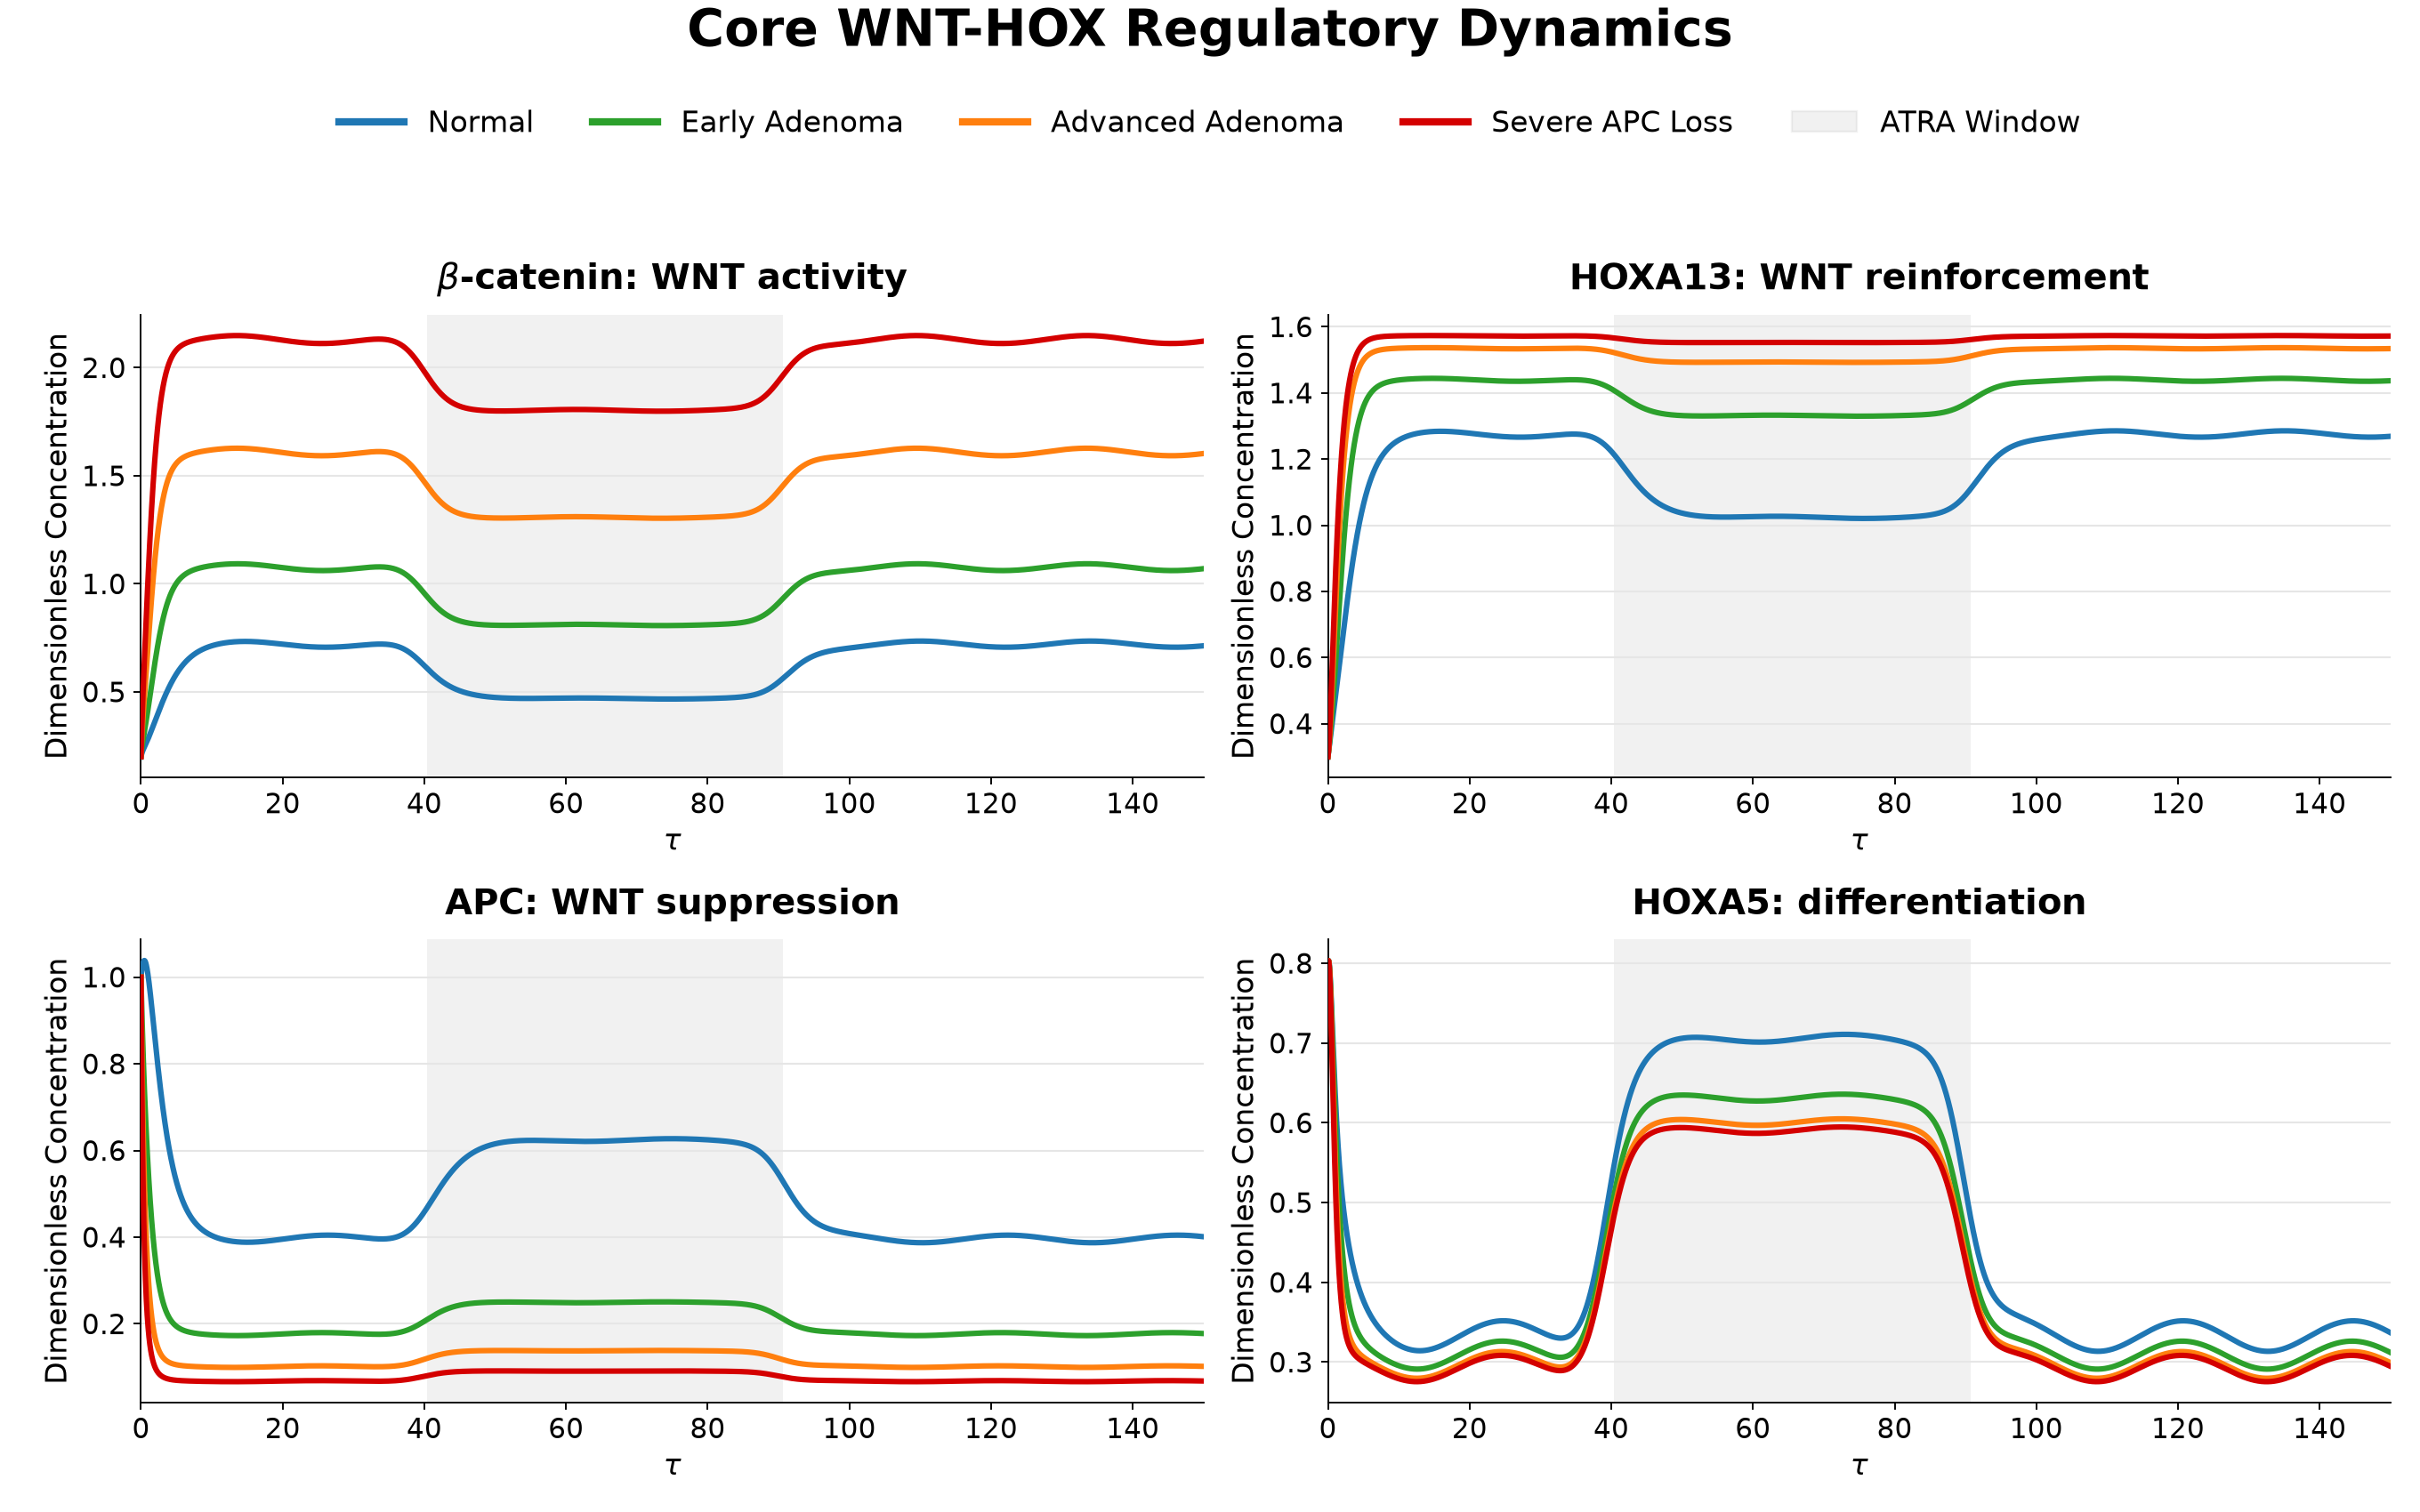
\includegraphics[height=8.12cm]{assets/scipy_core_dynamics.png}
\end{frame}

% 8 — Forward PINN architecture
\begin{frame}[plain]
  \centering
  \vspace{0.34cm}
  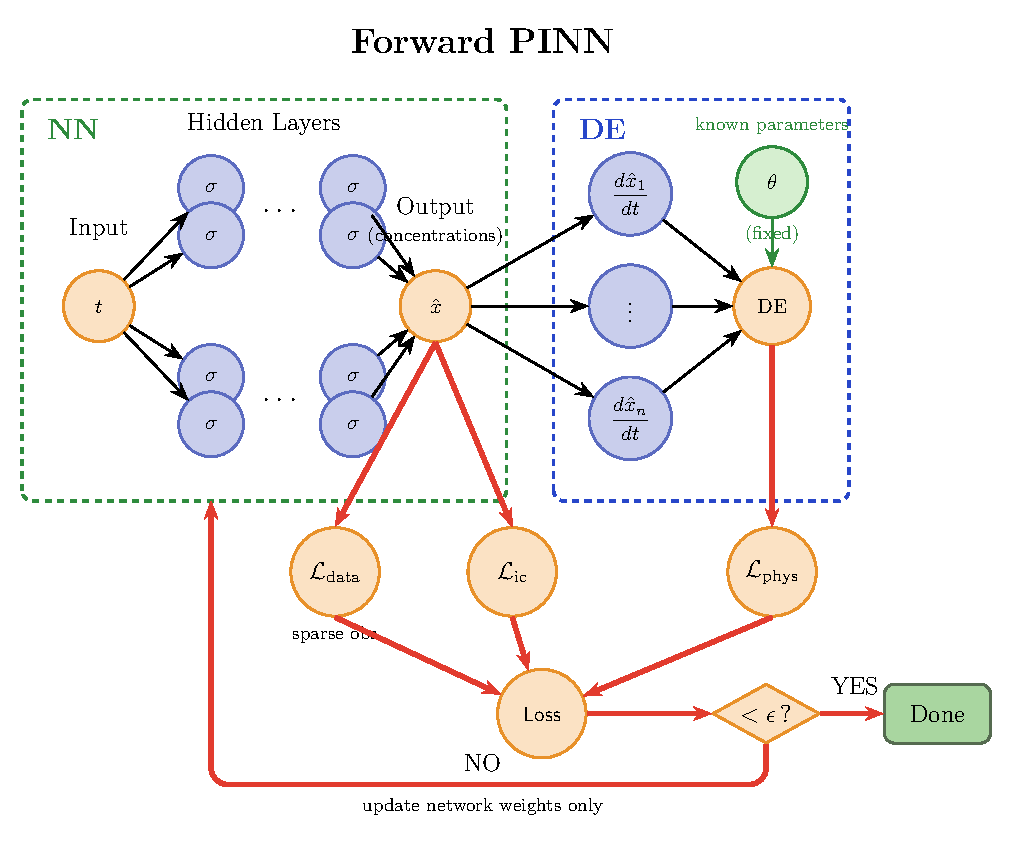
\includegraphics[height=8.20cm]{assets/forward_architecture.pdf}
\end{frame}

% 9 — Forward loss
\begin{frame}{Forward PINN Loss}
  \centering
  \vspace{0.06cm}
  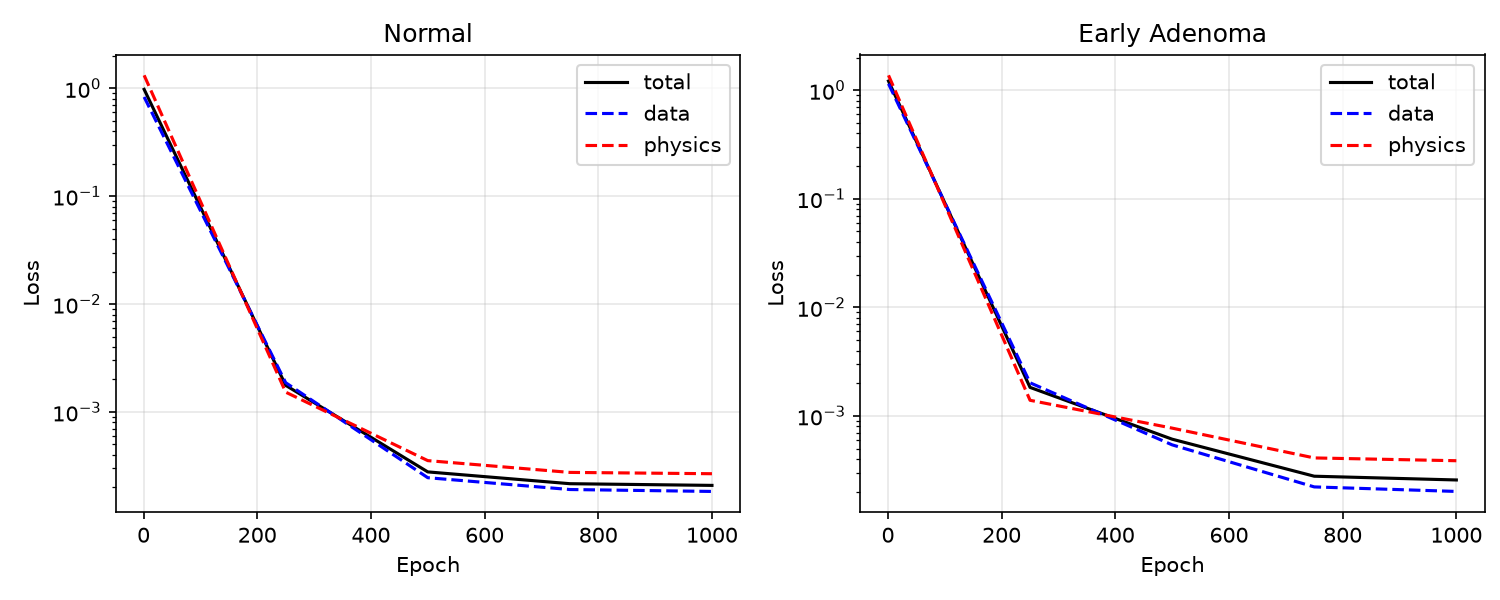
\includegraphics[width=0.59\textwidth]{assets/forward_losses_top.png}\par
  \vspace{0.08cm}
  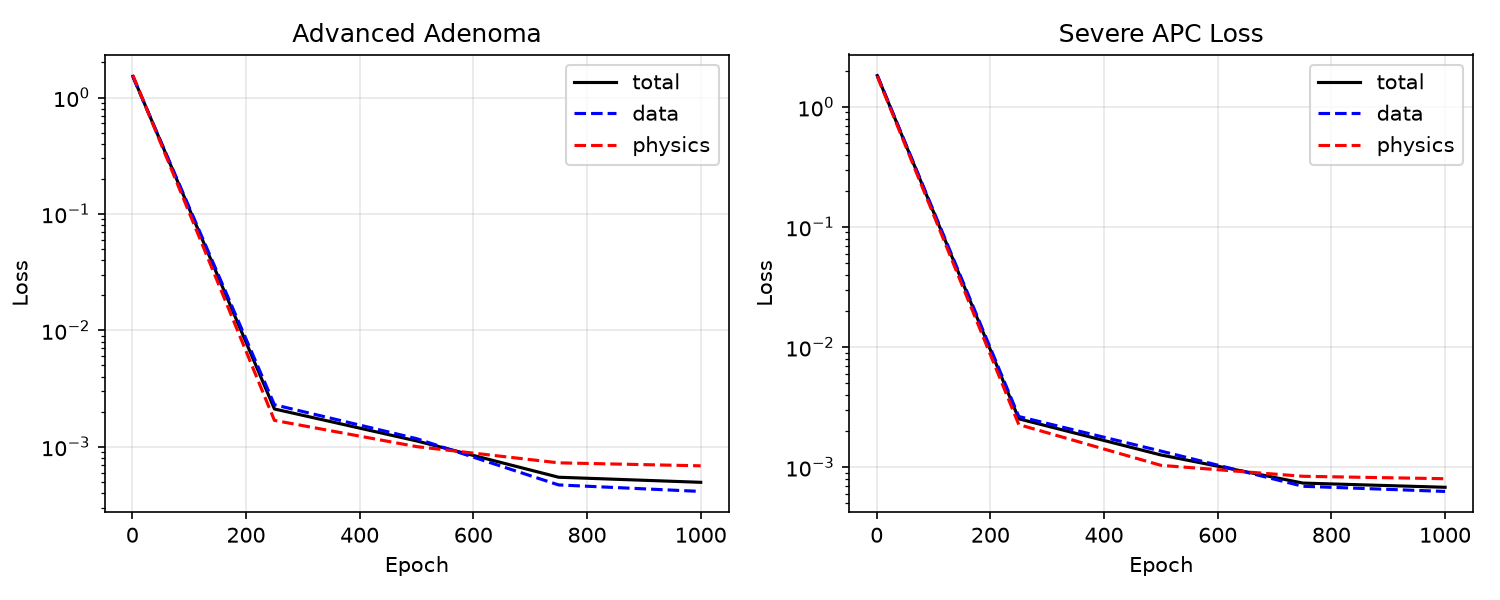
\includegraphics[width=0.59\textwidth]{assets/forward_losses_bottom.png}
\end{frame}

% 10 — Forward trajectories
\begin{frame}[plain]
  \centering
  \vspace{0.38cm}
  
\includegraphics[height=8.12cm]{assets/pinn_forward_core_dynamics.png}
\end{frame}

% 11 — Inverse PINN architecture
\begin{frame}[plain]
  \centering
  \vspace{0.34cm}
  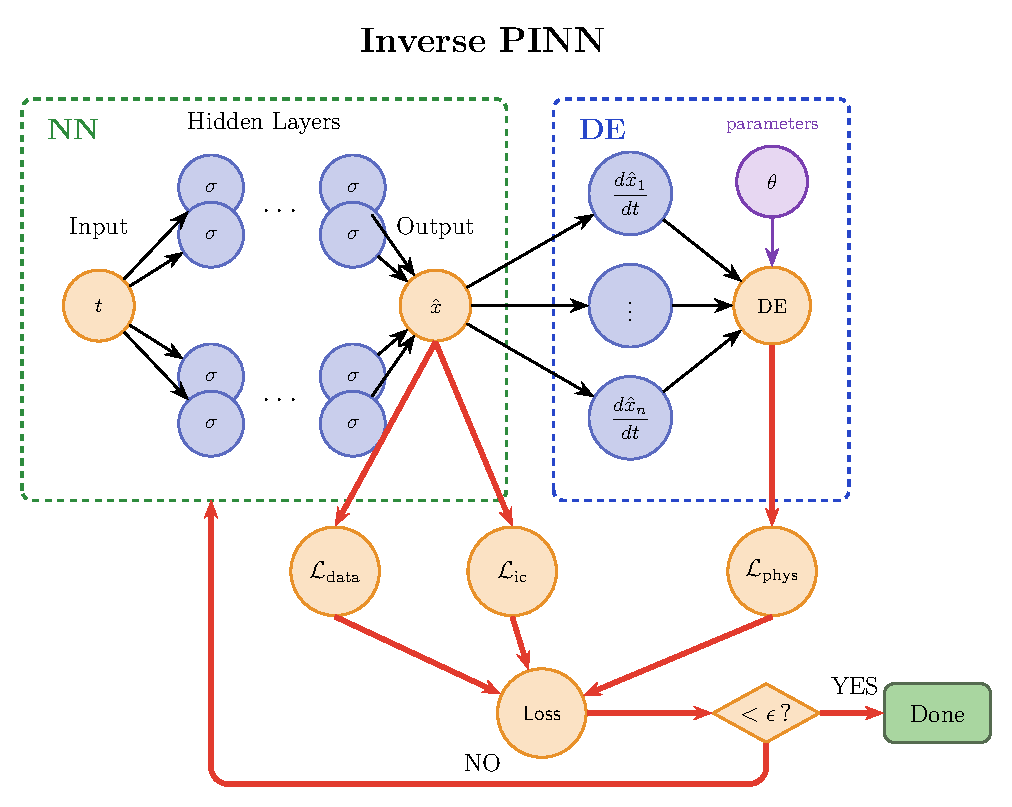
\includegraphics[height=8.20cm]{assets/inverse_architecture.pdf}
\end{frame}

% 12 — Inverse loss
\begin{frame}{Inverse PINN Loss}
  \centering
  \vspace{0.06cm}
  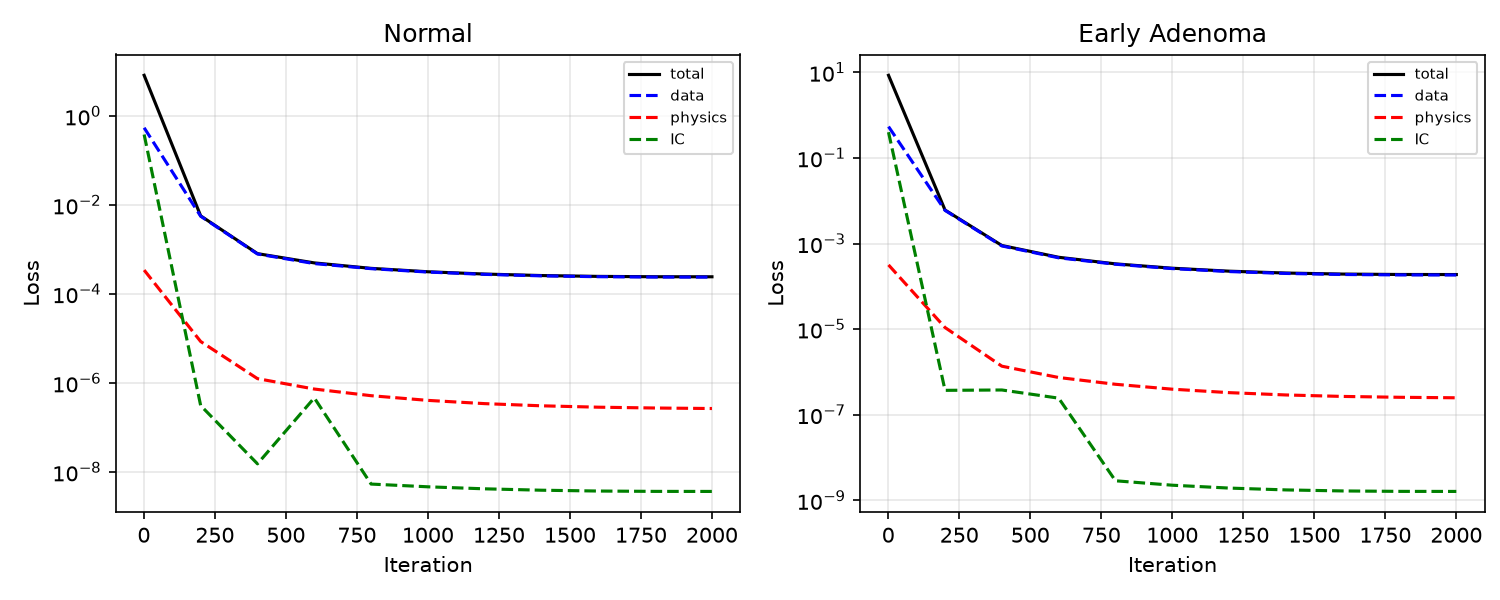
\includegraphics[width=0.59\textwidth]{assets/inverse_losses_top.png}\par
  \vspace{0.08cm}
  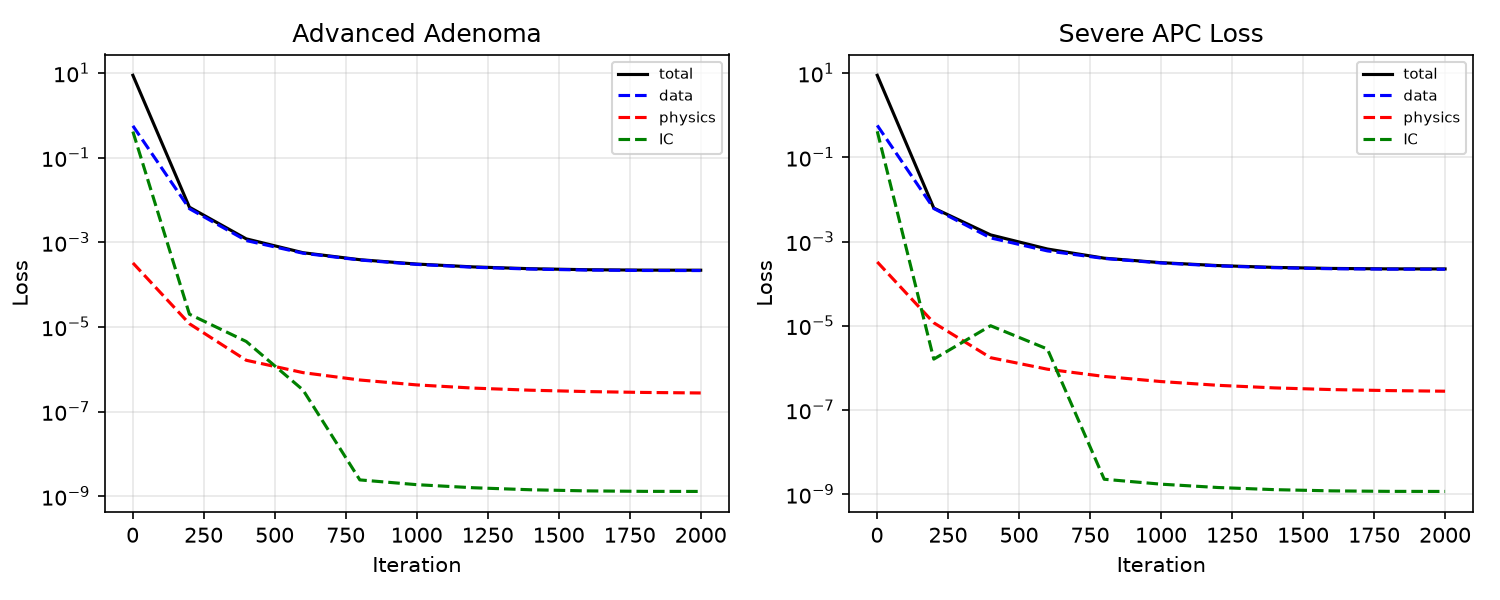
\includegraphics[width=0.59\textwidth]{assets/inverse_losses_bottom.png}
\end{frame}

% 13 — Inverse trajectories
\begin{frame}[plain]
  \centering
  \vspace{0.38cm}
  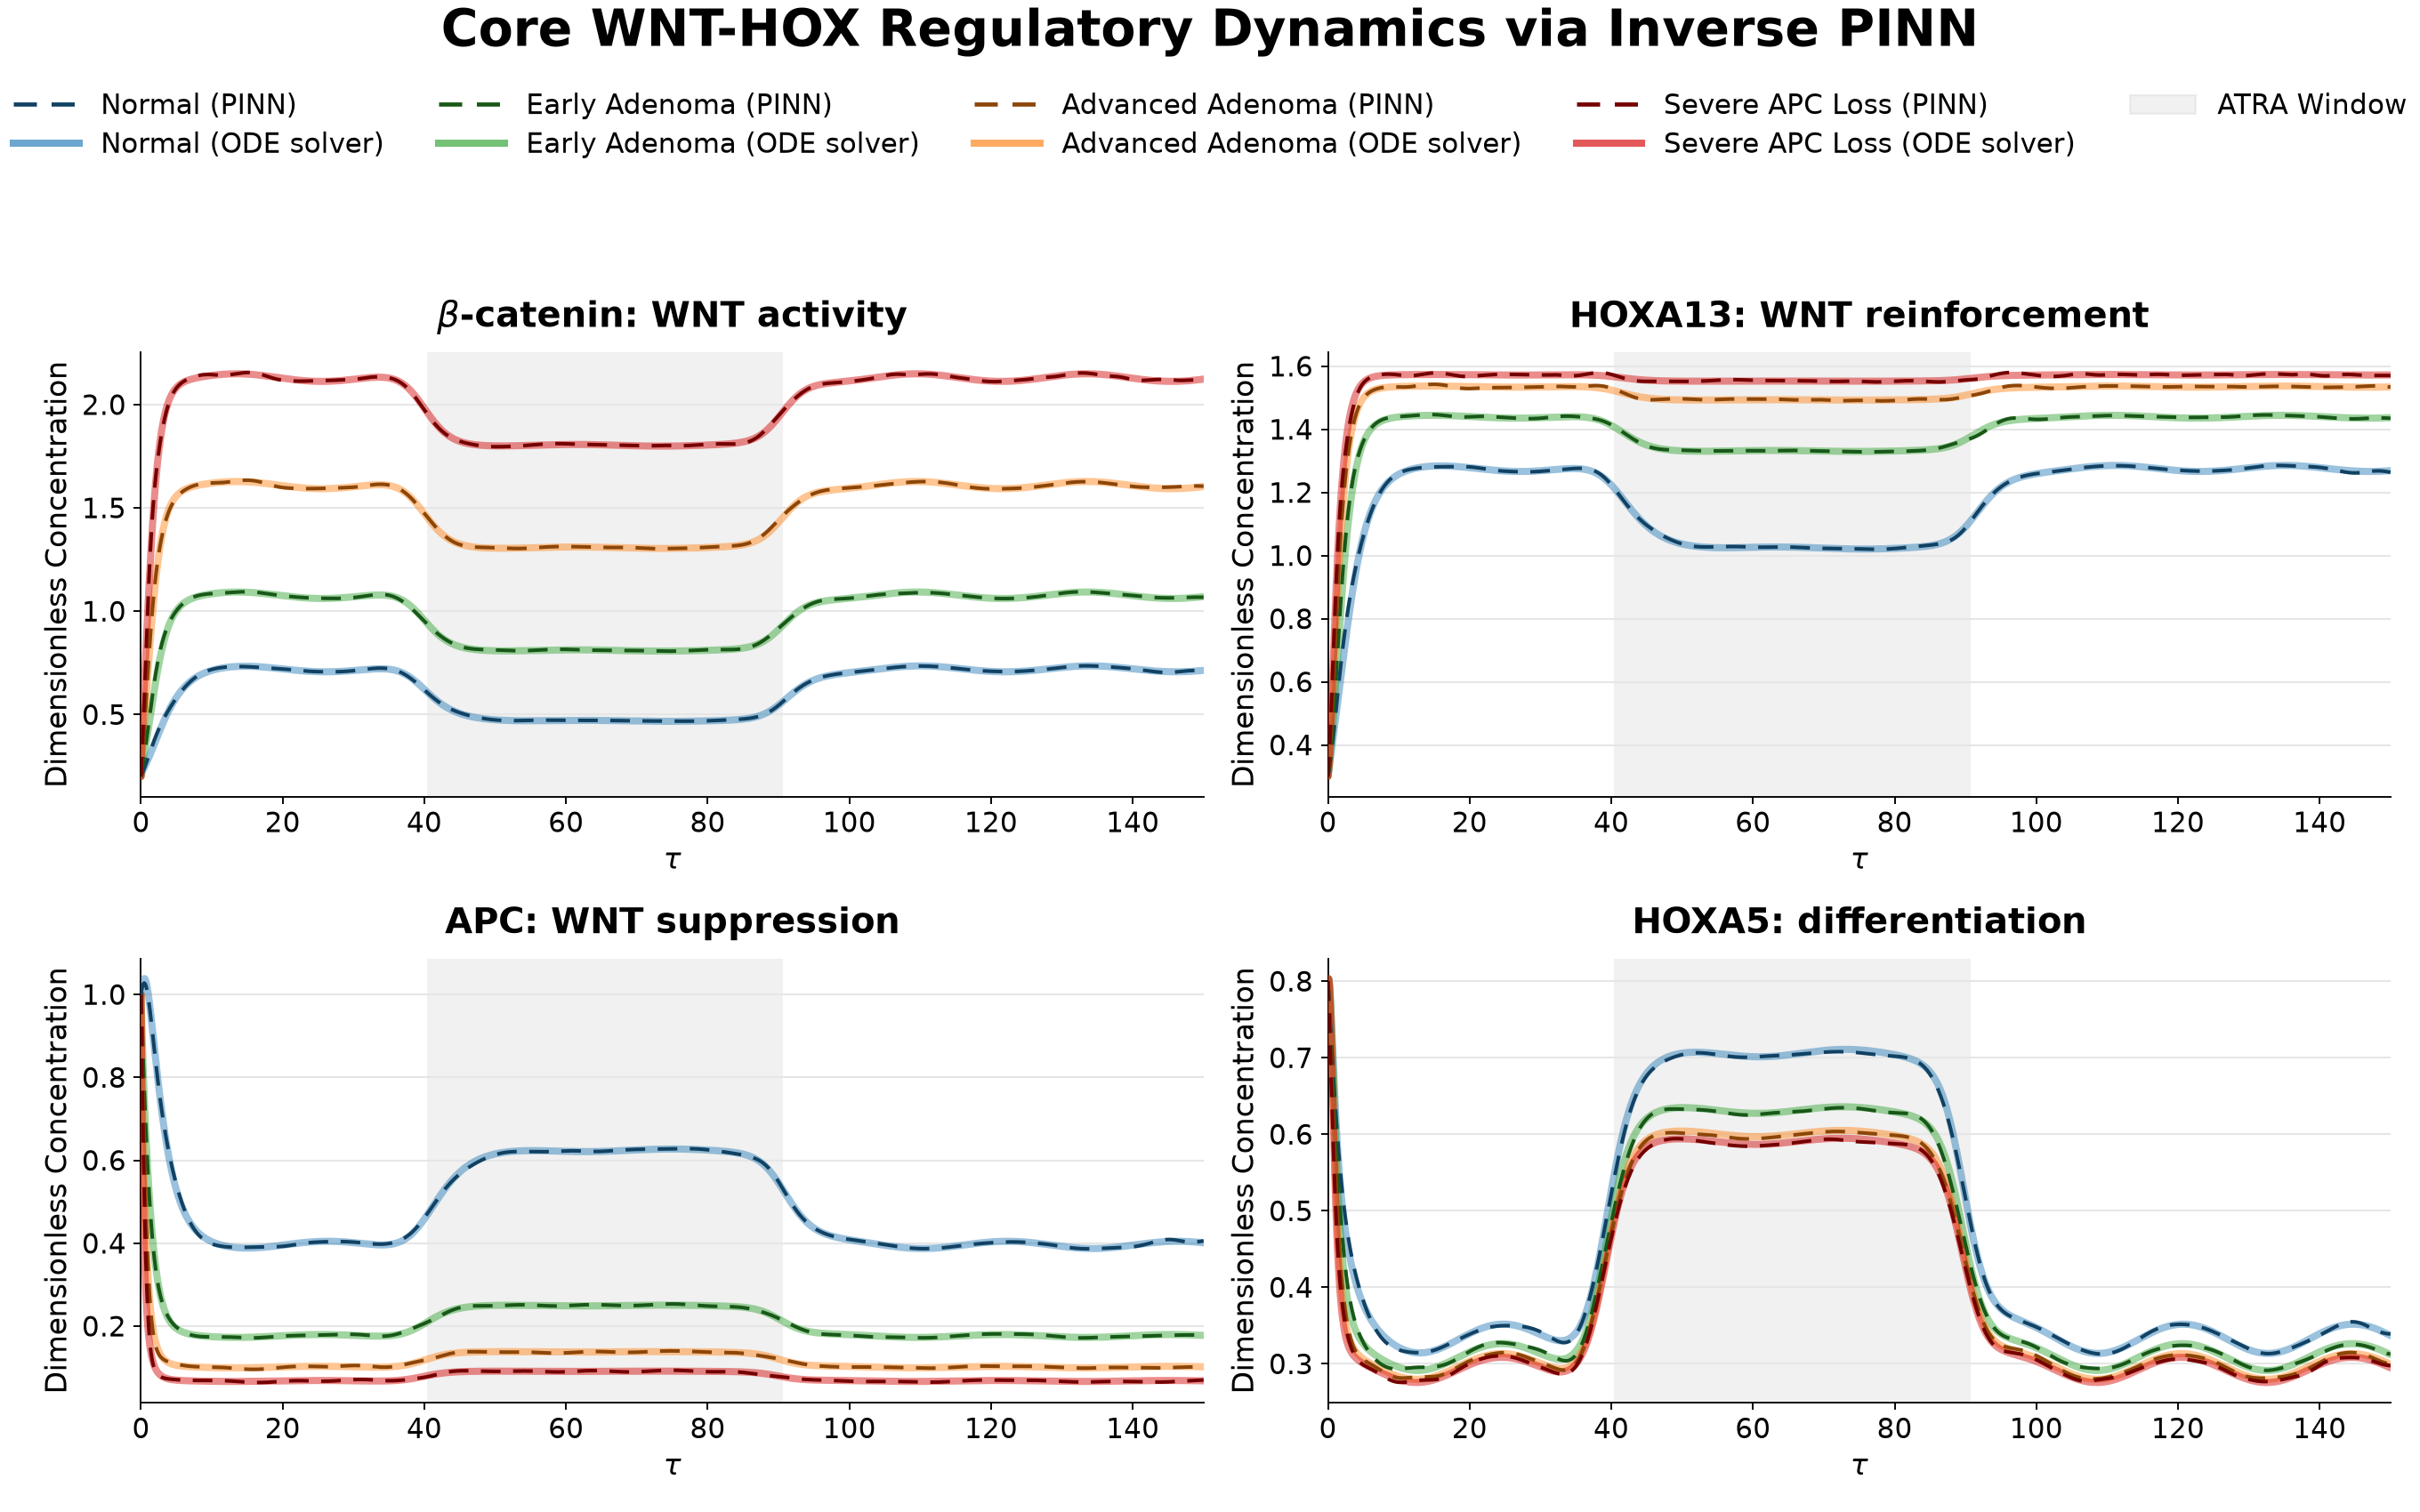
\includegraphics[height=8.12cm]{assets/pinn_inverse_core_dynamics.png}
\end{frame}

% 14 — Parameter recovery bars
\begin{frame}[plain]
  \centering
  \vspace{0.35cm}
  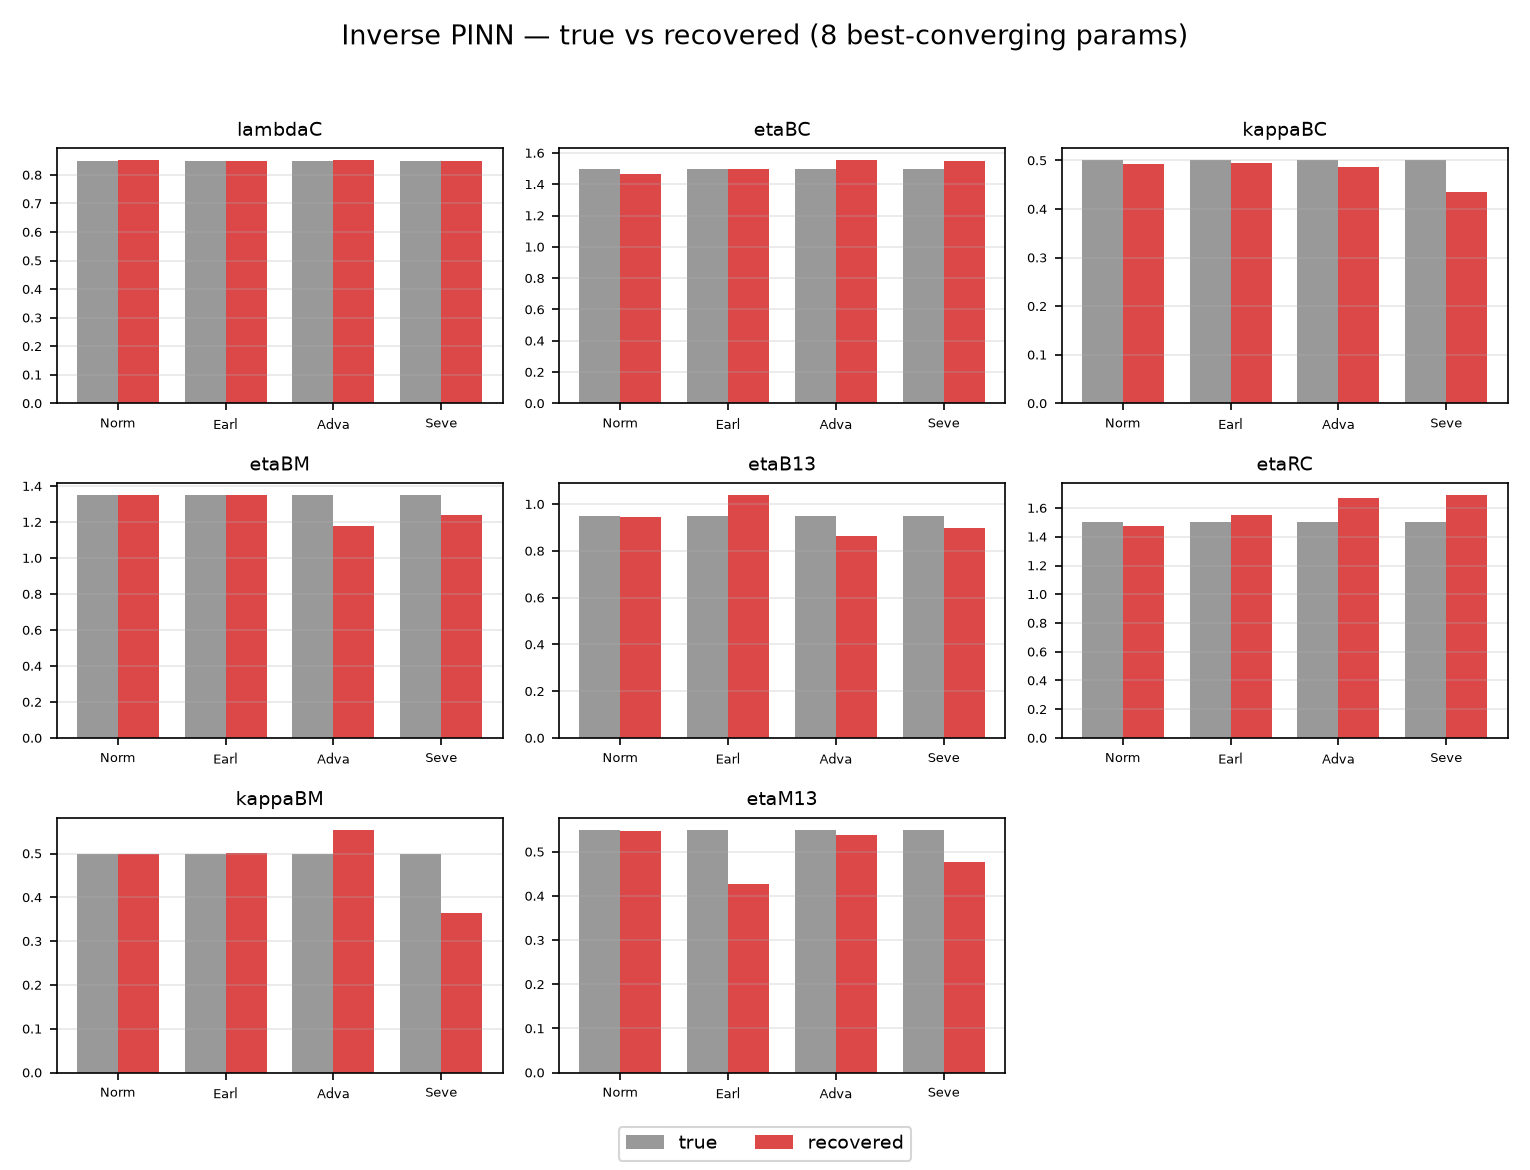
\includegraphics[height=8.18cm]{assets/inverse_recovery_bars_best8.png}
\end{frame}

% 15 — Bayesian normal
\begin{frame}{Inverse Bayesian PINN - uncertainty quantification}
  \centering
  \vspace{0.20cm}
  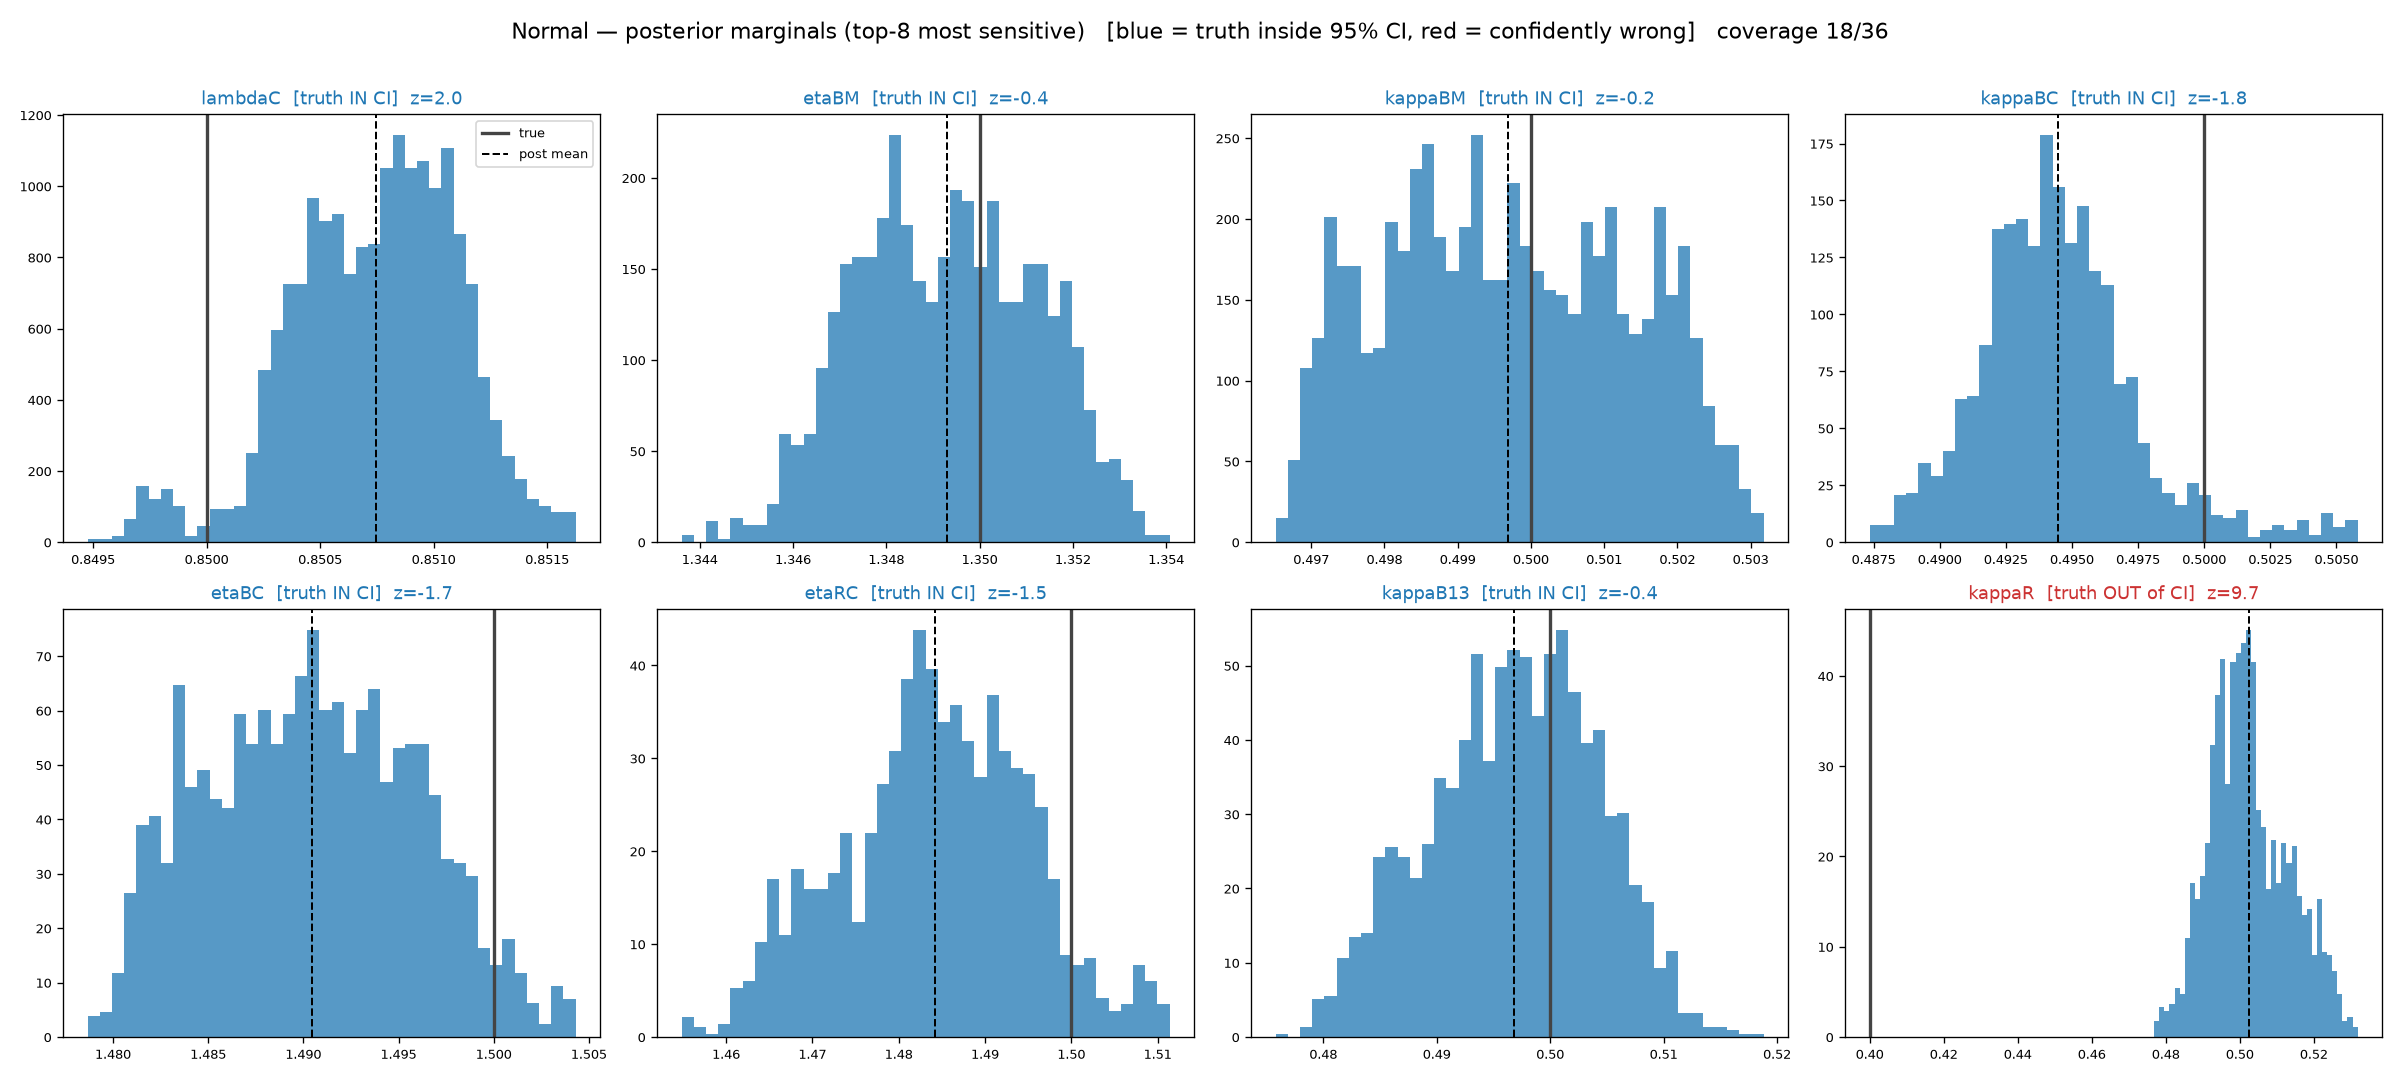
\includegraphics[width=0.96\textwidth]{assets/normal_top8_marginals.png}
\end{frame}

% 16 — Bayesian severe
\begin{frame}{Inverse Bayesian PINN - continued}
  \centering
  \vspace{0.20cm}
  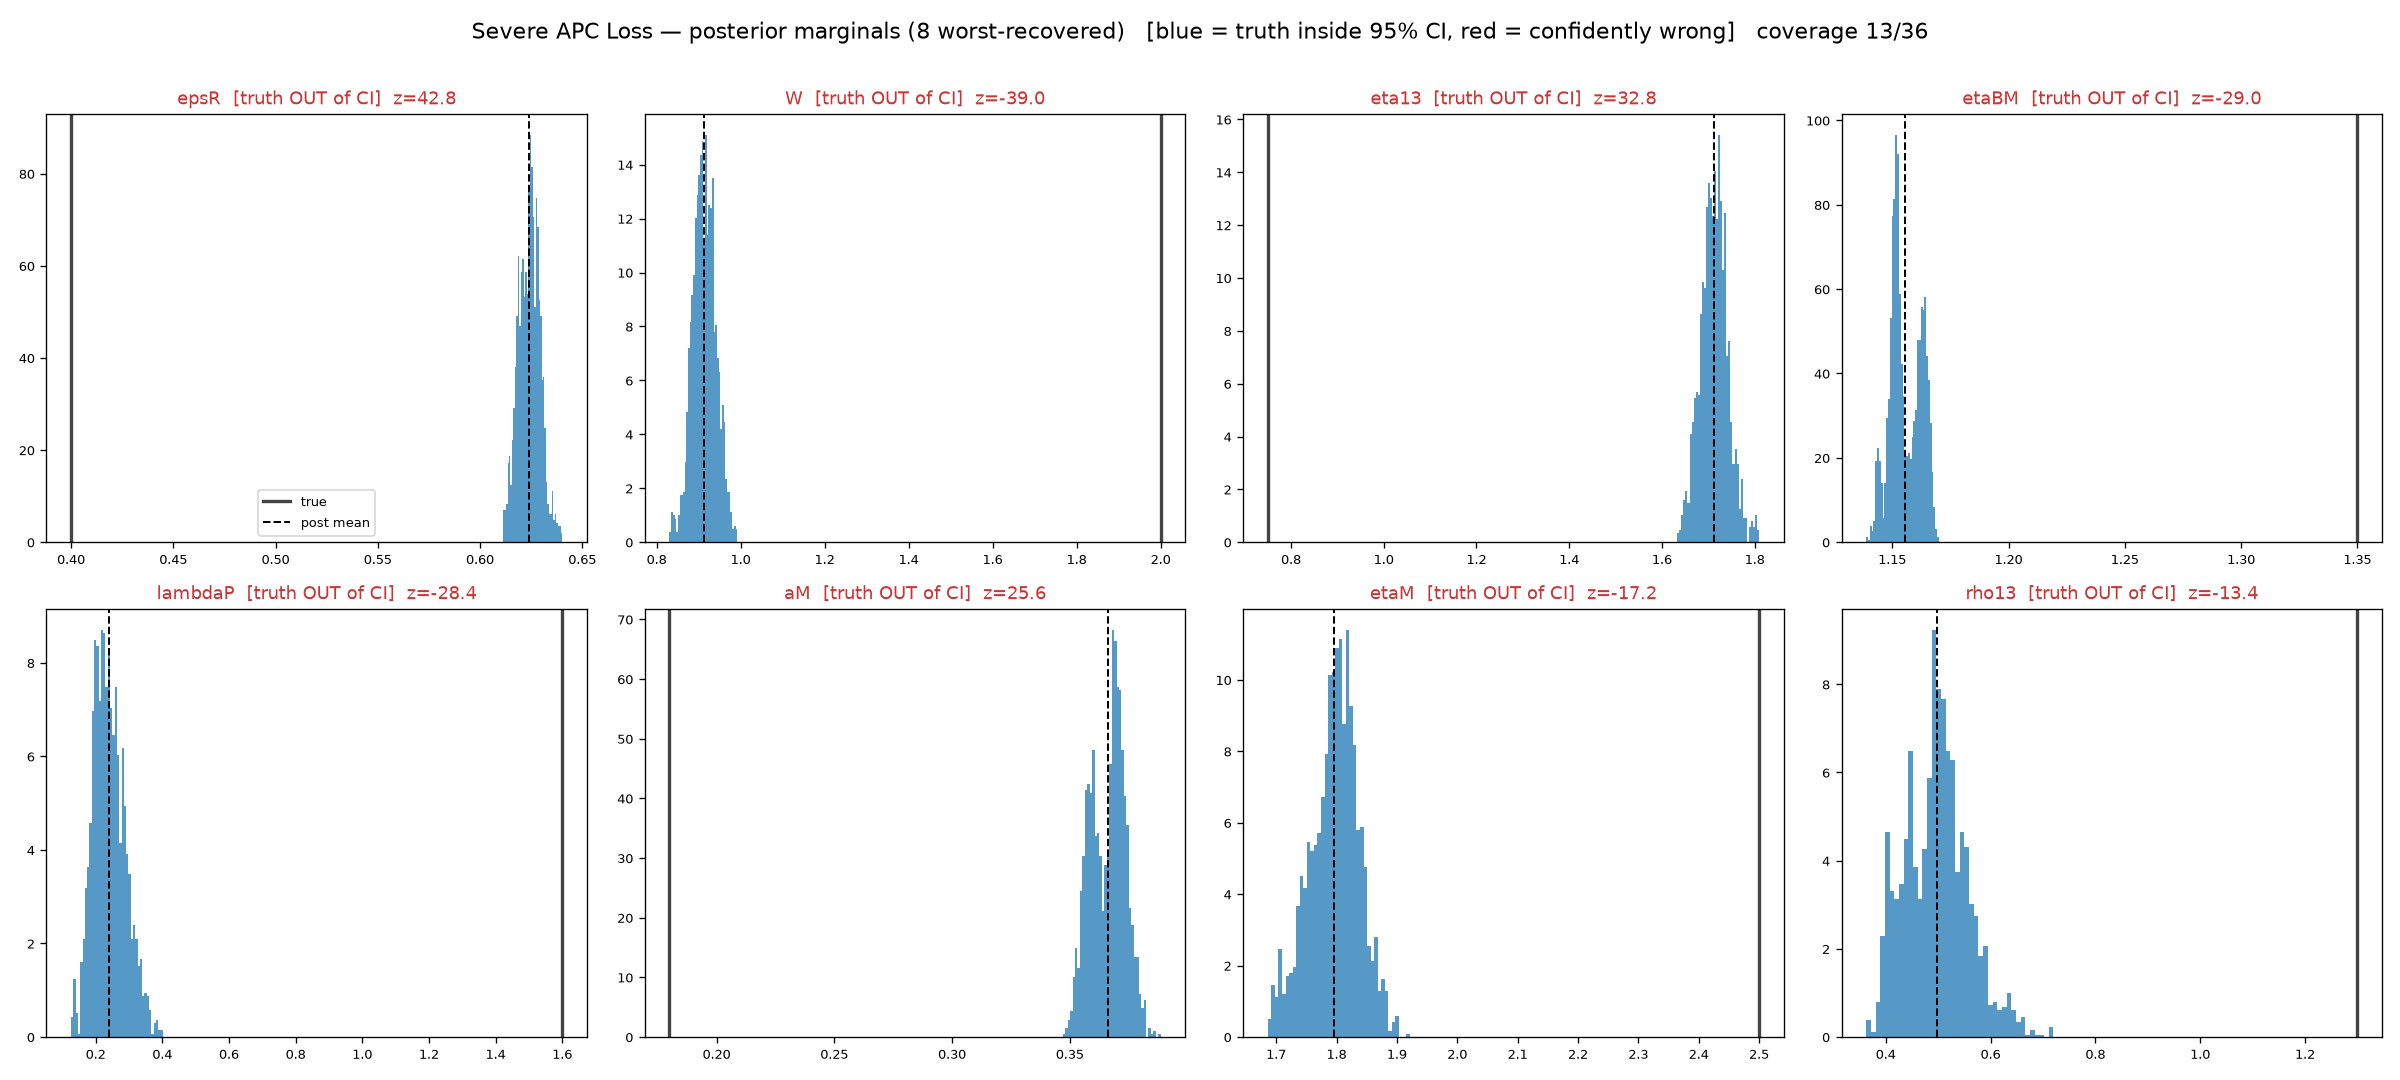
\includegraphics[width=0.96\textwidth]{assets/severe_worst8_marginals.png}
\end{frame}

% 17 — Comparison table
\begin{frame}{Parameter Recovery Comparison}
  \vspace{0.28cm}
  \renewcommand{\arraystretch}{1.52}
  \arrayrulecolor{Cobalt}
  \begin{tabularx}{\textwidth}{@{}Xccc@{}}
    \toprule
    \rowcolor{TintWarm}
    & \textbf{Bayesian inverse PINN} & \textbf{Inverse PINN} & \textbf{ODE-fit} \\
    \midrule
    % Garnet marks the BEST recovery count in each row, not a fixed column:
    % the Bayesian PINN wins the two low-WNT regimes, the ODE-fit the two
    % high-WNT ones.
    ``Normal'' & \best{19} & 17 & 18/36 \\
    \rowcolor{Tint}
    ``Early Adenoma'' & \best{20} & 16 & 17/36 \\
    ``Advanced Adenoma'' & 11 & 10 & \best{13/36} \\
    \rowcolor{Tint}
    ``Severe APC Loss'' & 8 & 7 & \best{11/36} \\
    \bottomrule
  \end{tabularx}
  \arrayrulecolor{black}
\end{frame}

% 18 — Next steps
\begin{frame}{Next Steps}
  \begin{columns}[c,totalwidth=\textwidth]
    \begin{column}{0.49\textwidth}
      \begin{itemize}\setlength\itemsep{0.30cm}
        \item Improve Bayesian PINN
          \begin{itemize}\item Investigate limitations\end{itemize}
        \item Hybrid Mechanistic-Neural Model
        \item Stochastic Modeling
      \end{itemize}
    \end{column}
    \begin{column}{0.47\textwidth}
      \centering\imagepanel[width=0.96\linewidth]{assets/source_next_steps.jpg}
    \end{column}
  \end{columns}
\end{frame}

% 19 — References
\begin{frame}[plain]
  \centering
  \vspace{0.16cm}
  {\fontsize{15}{18}\selectfont\bfseries\color{Ink}Key References\par}
  \vspace{0.08cm}
  {\color{Cobalt}\rule{0.965\textwidth}{1.4pt}}
  \vspace{0.10cm}

  \begin{minipage}{0.965\textwidth}
    \raggedright
    \fontsize{9.6}{13.0}\selectfont
    \renewcommand{\arraystretch}{1.06}
    % The one-line \refwhy{} annotations under each entry are commented out
    % for now (kept verbatim so they can be switched back on); font size and
    % row spacing above were enlarged to fill the slide without them.
    \begin{tabular}{@{}p{0.75cm}@{}p{\dimexpr\linewidth-0.75cm\relax}@{}}
      \refnum{1.} & \textbf{Raissi, Perdikaris \& Karniadakis (2019).}
        Physics-informed neural networks: a deep learning framework for solving
        forward and inverse problems involving nonlinear PDEs.
        \emph{J.\ Comput.\ Phys.} \textbf{378}, 686--707.\\[5.5pt]
      %      & \refwhy{Foundational PINN formulation --- the data + physics-residual loss used in every model here.}\\[1.8pt]

      \refnum{2.} & \textbf{Yazdani, Lu, Raissi \& Karniadakis (2020).}
        Systems biology informed deep learning for inferring parameters and
        hidden dynamics. \emph{PLoS Comput.\ Biol.} \textbf{16}(11), e1007575.\\[5.5pt]
      %      & \refwhy{Closest template to this work: inverse PINNs on biological ODE networks; the local-sensitivity/Fisher route to identifiability.}\\[1.8pt]

      \refnum{3.} & \textbf{Yang, Meng \& Karniadakis (2021).}
        B-PINNs: Bayesian physics-informed neural networks for forward and
        inverse PDE problems with noisy data.
        \emph{J.\ Comput.\ Phys.} \textbf{425}, 109913.\\[5.5pt]
      %      & \refwhy{Basis of the Bayesian inverse PINN: HMC over parameters gives posterior marginals instead of a point estimate.}\\[1.8pt]

      \refnum{4.} & \textbf{Raue \emph{et al.} (2009).}
        Structural and practical identifiability analysis of partially observed
        dynamical models by exploiting the profile likelihood.
        \emph{Bioinformatics} \textbf{25}(15), 1923--1929.\\[5.5pt]
      %      & \refwhy{The identifiability verdict --- profile likelihood distinguishes the structural from the practical (high-WNT $\theta_P$) wall.}\\[1.8pt]

      \refnum{5.} & \textbf{Wang, Yu \& Perdikaris (2022).}
        When and why PINNs fail to train: a neural tangent kernel perspective.
        \emph{J.\ Comput.\ Phys.} \textbf{449}, 110768.\\[5.5pt]
      %      & \refwhy{Explains the loss-term imbalance and spectral bias behind the training pathologies; motivates adaptive loss weighting.}\\[1.8pt]

      \refnum{6.} & \textbf{Tancik \emph{et al.} (2020).}
        Fourier features let networks learn high frequency functions in low
        dimensional domains. \emph{NeurIPS} \textbf{33}, 7537--7547.\\[5.5pt]
      %      & \refwhy{Fourier-feature time embedding --- required to capture the circadian RA forcing and the ATRA pulse.}\\[1.8pt]

      \refnum{7.} & \textbf{Ji, Qiu, Zhang \& Deng (2021).}
        Stiff-PINN: physics-informed neural network for stiff chemical kinetics.
        \emph{J.\ Phys.\ Chem.\ A} \textbf{125}(36), 8098--8106.
      %      & \refwhy{Diagnoses PINN failure on stiff multiscale kinetics --- the same stiffness that shapes the WNT--RA--HOX residual.}\\
    \end{tabular}
  \end{minipage}
\end{frame}

% 20 — Thank you
\begin{frame}{Thank you!}
  \centering
  {\large Questions? (we will try to answer)}\hspace{0.14cm}
\includegraphics[height=0.42cm]{assets/source_emoji.jpg}
  \vspace{0.18cm}
  \begin{columns}[T,totalwidth=\textwidth]
    \begin{column}{0.46\textwidth}
      \centering
      {\scriptsize PK calling Amir + Nate to check in on our progress\ldots}\par
      \vspace{0.10cm}
      
\includegraphics[height=1.35cm]{assets/source_advisor.jpg}
      \vspace{0.12cm}
      \begin{columns}[T,totalwidth=\linewidth]
        \begin{column}{0.49\linewidth}
          \centering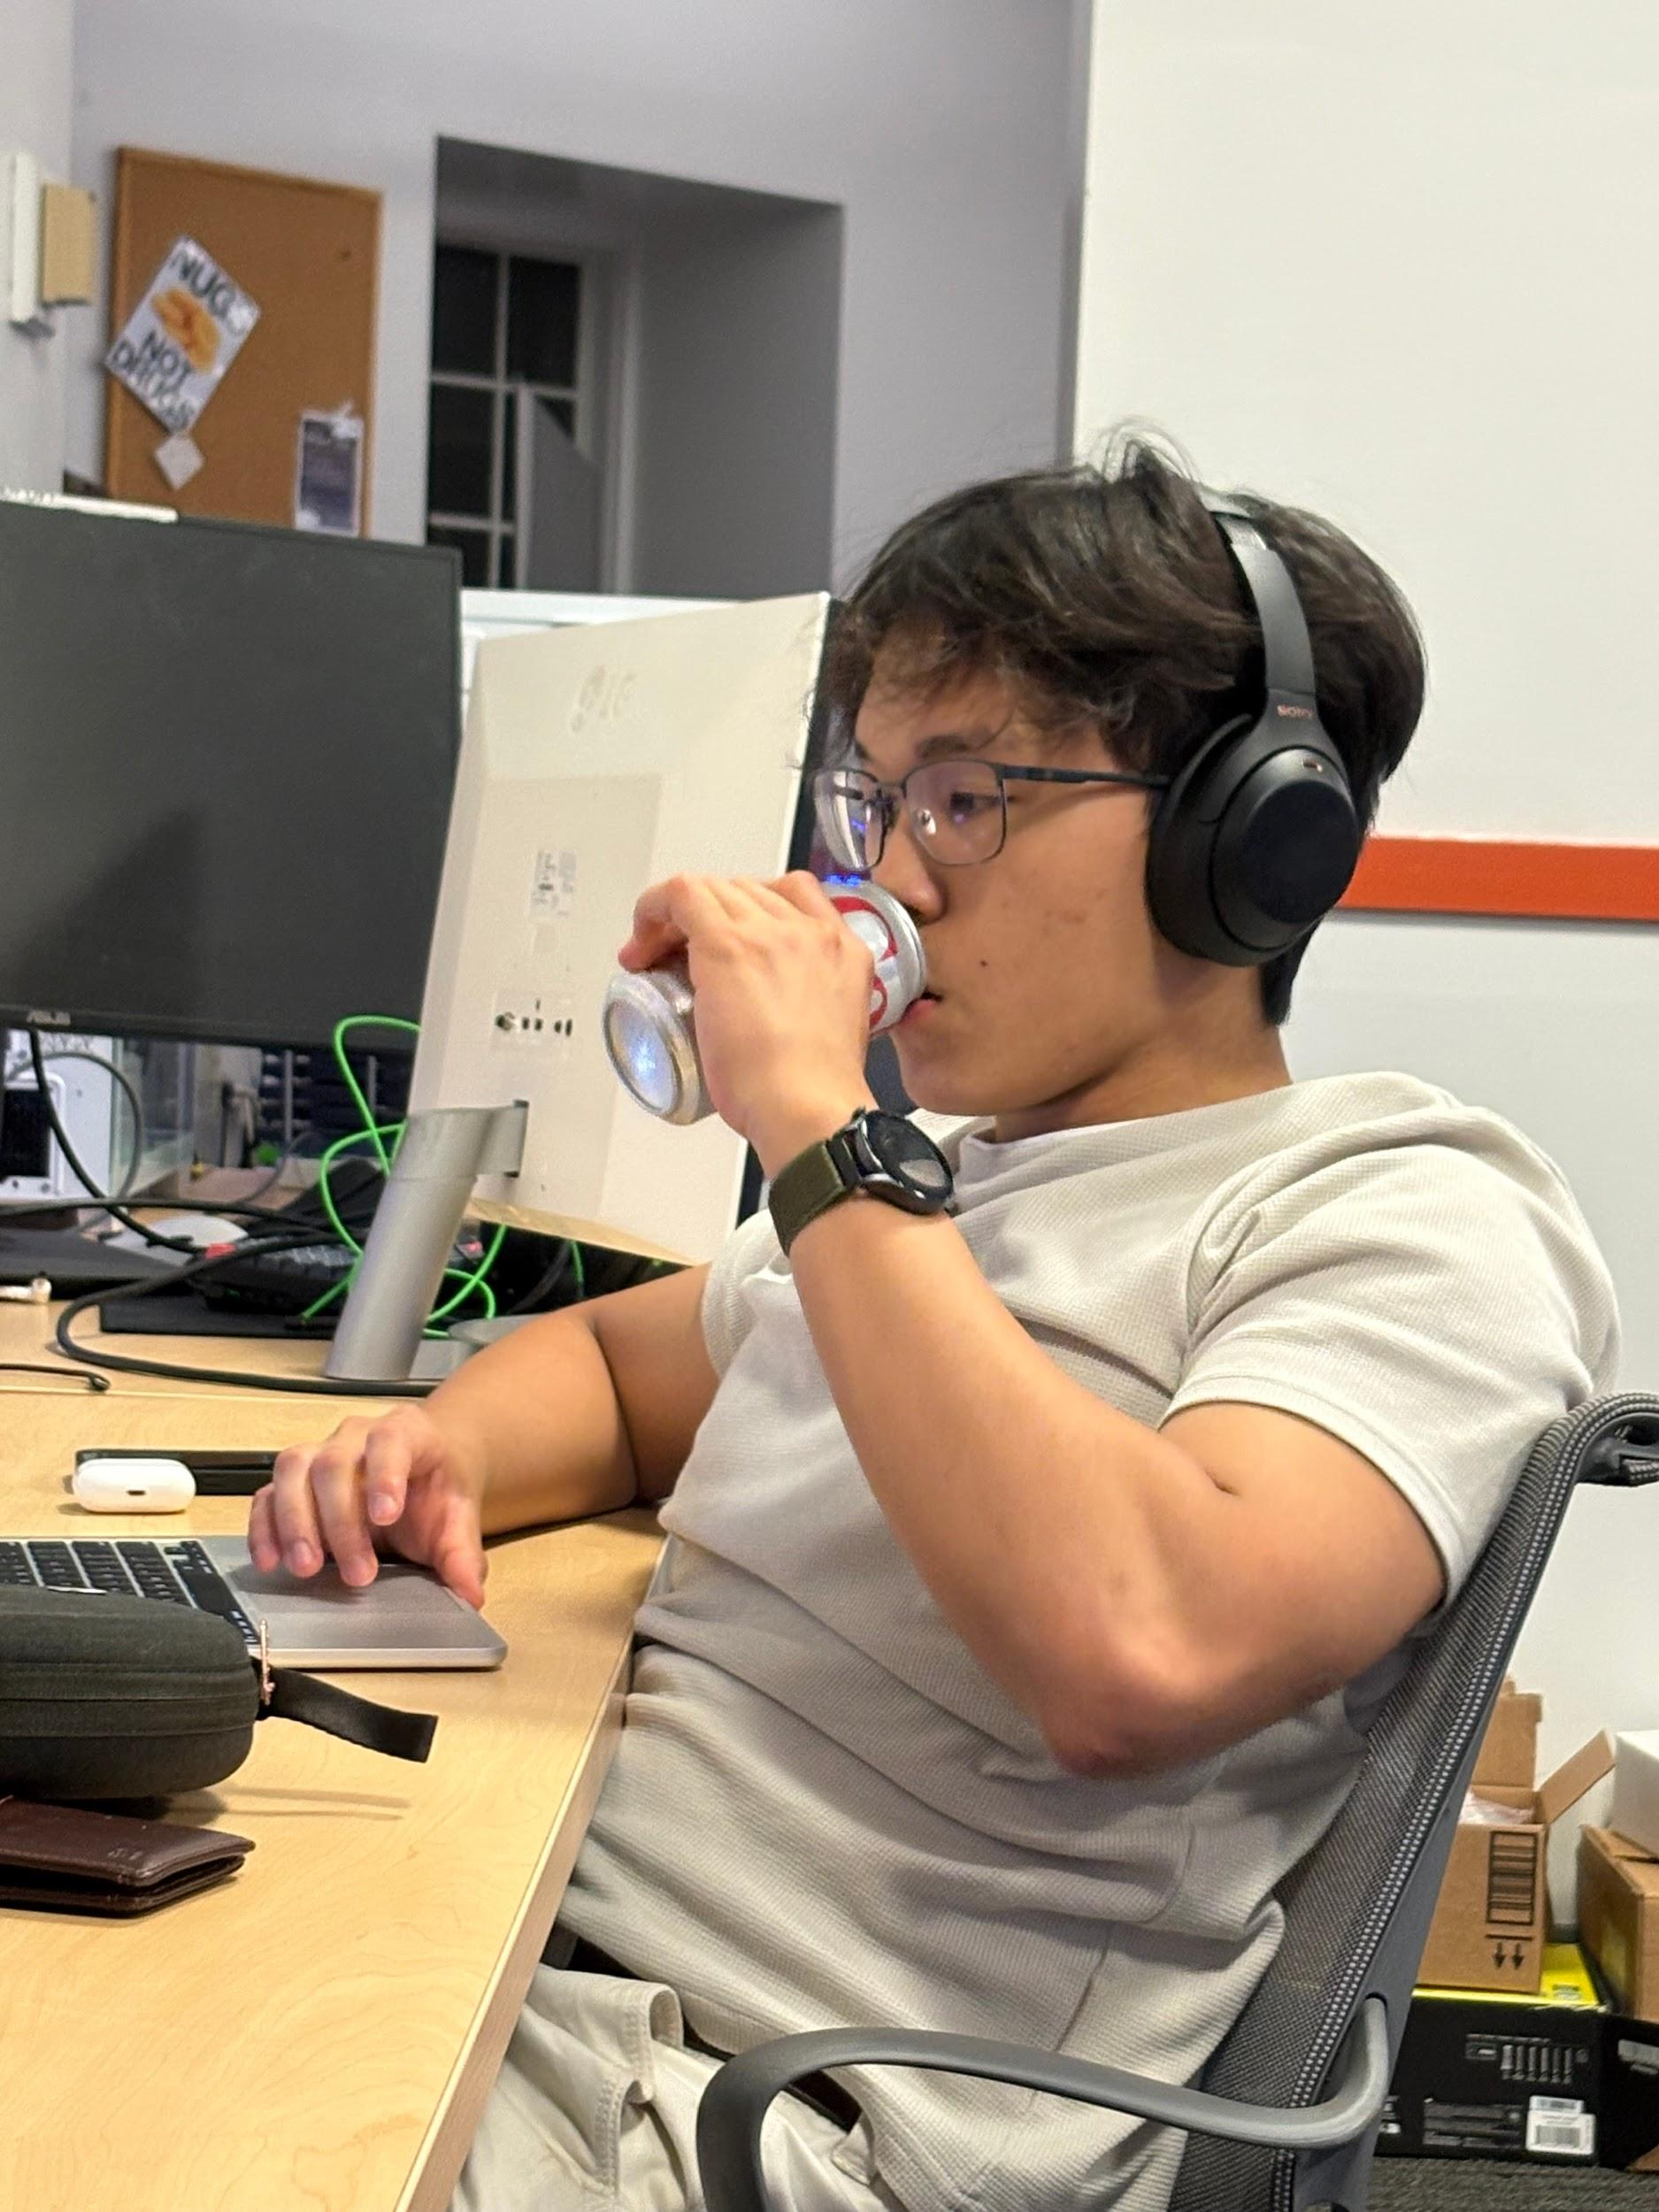
\includegraphics[height=1.95cm]{assets/source_nate.jpg}\par
          {\fontsize{5.2}{6.0}\selectfont 4th diet coke of the day + Celsius b/c his sleep schedule is so cooked}
        \end{column}
        \begin{column}{0.49\linewidth}
          \centering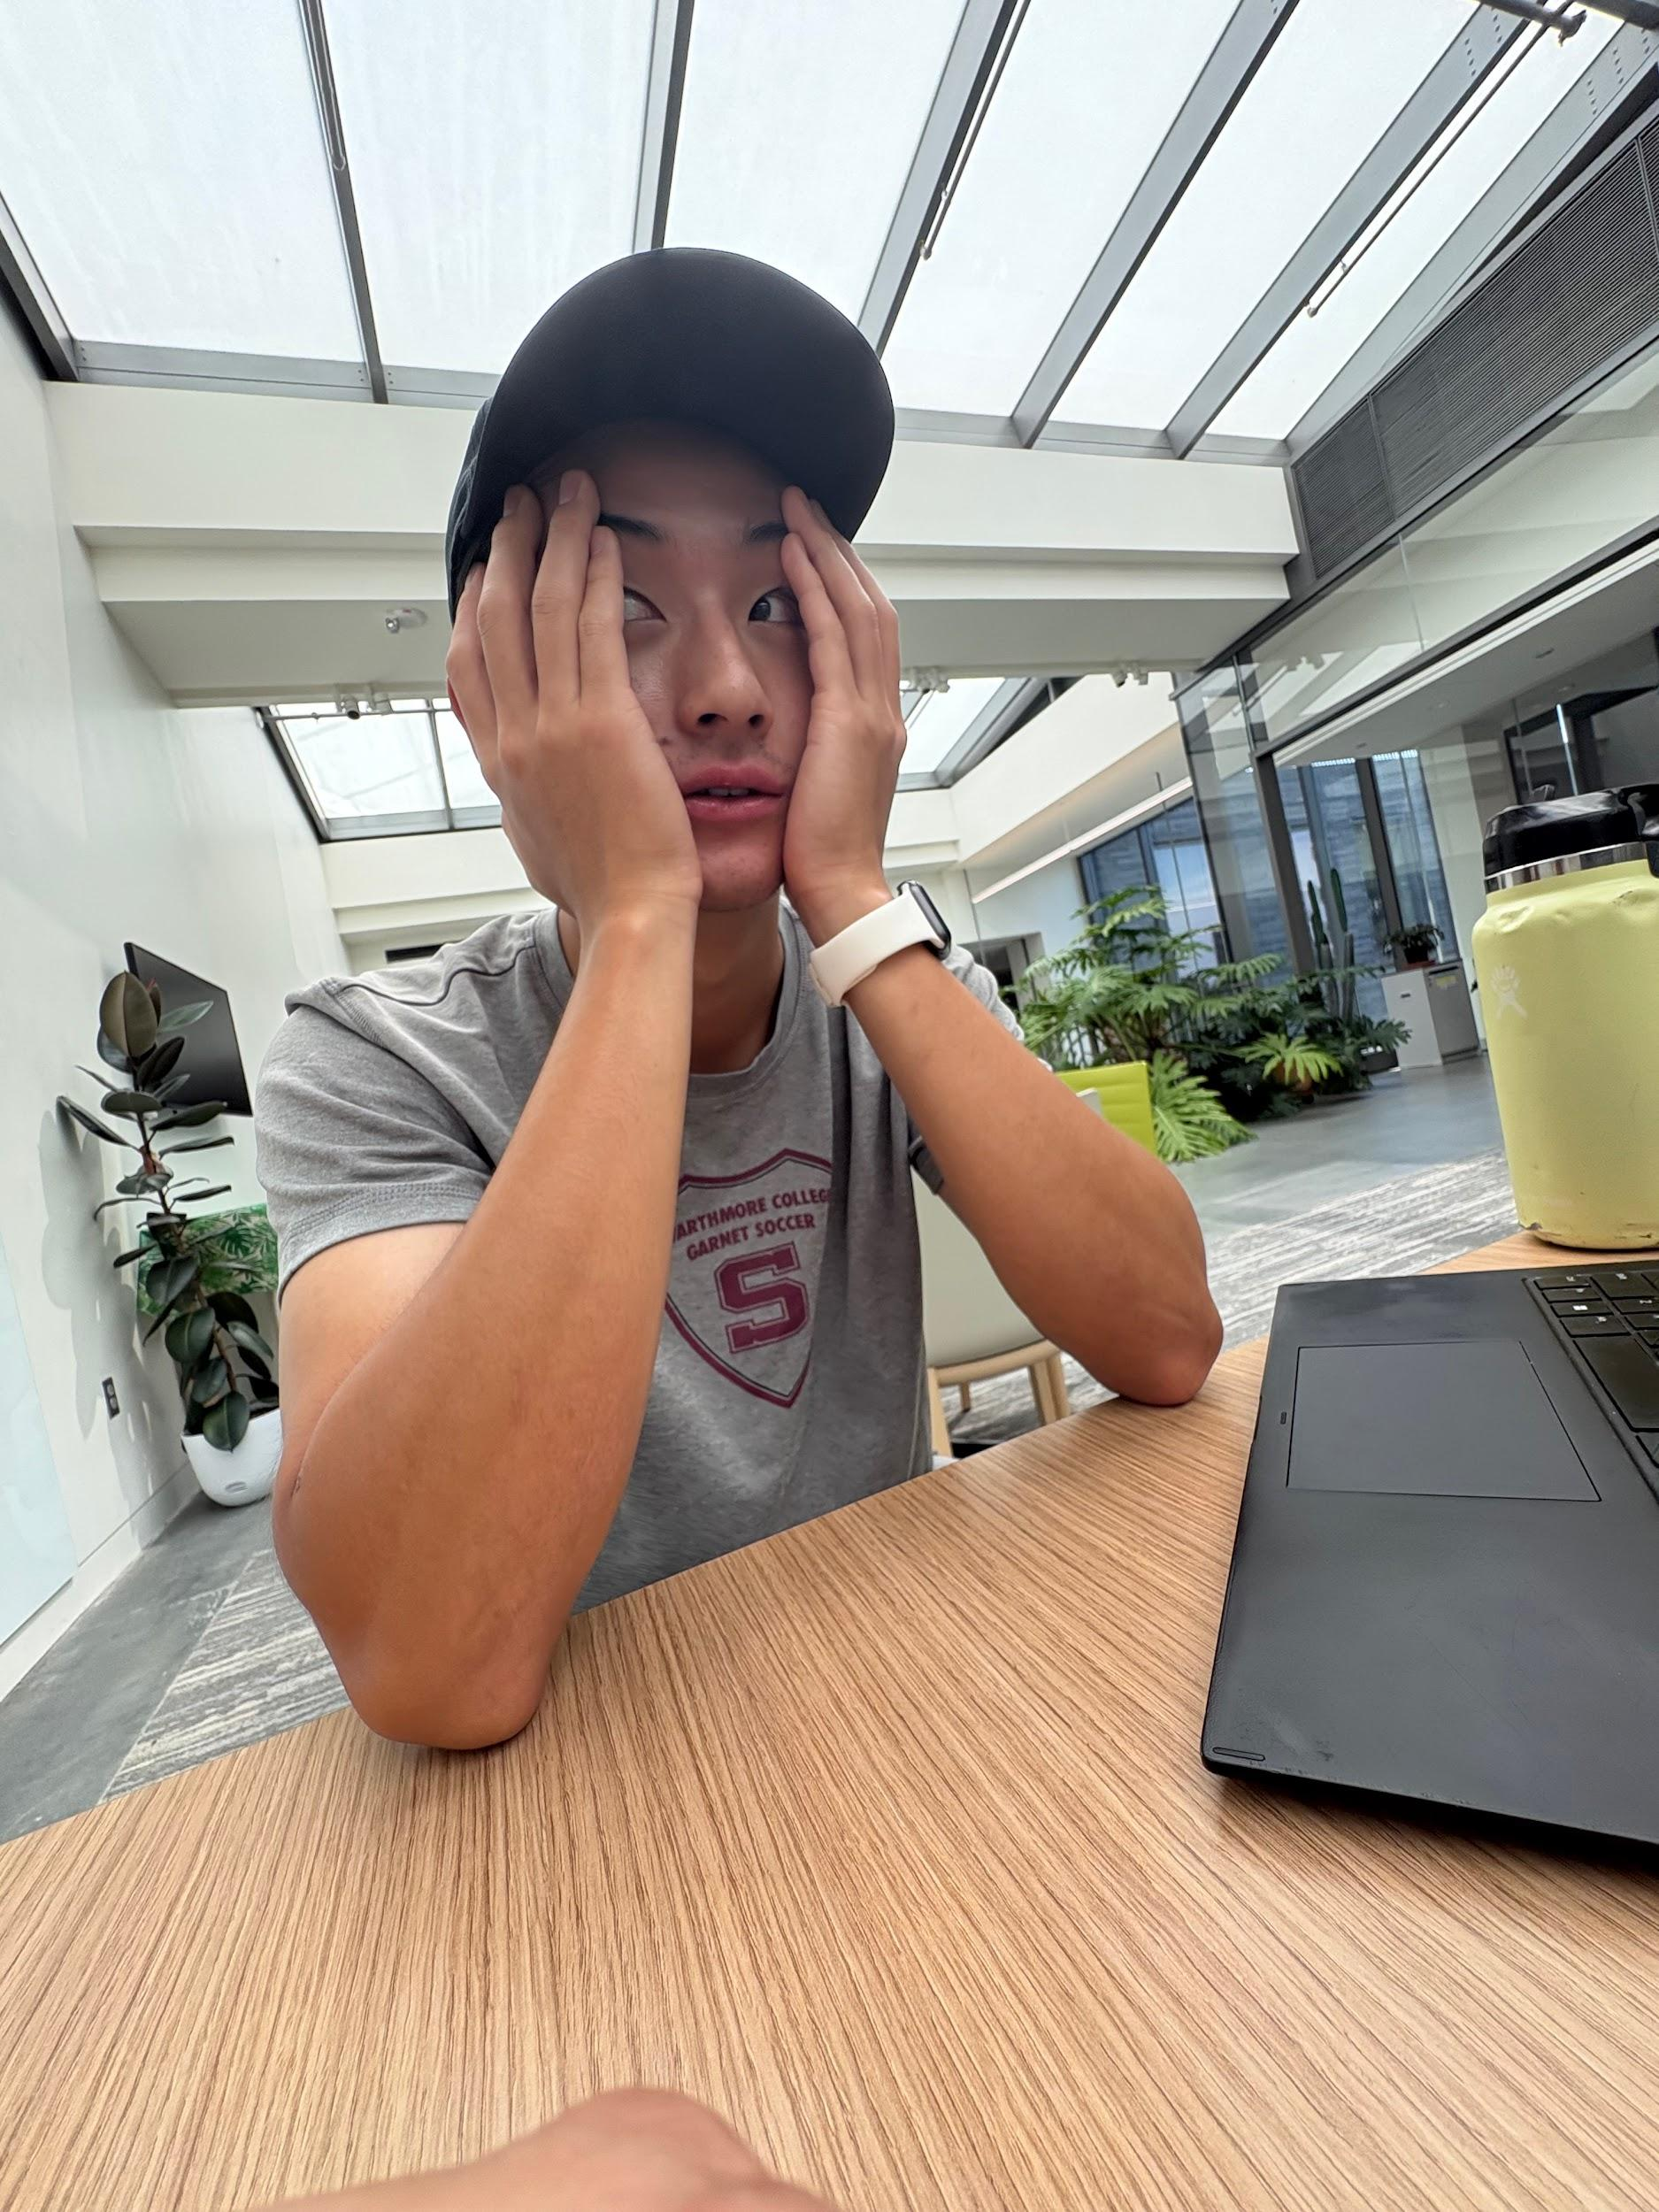
\includegraphics[height=1.95cm]{assets/source_amir.jpg}\par
          {\fontsize{5.2}{6.0}\selectfont Don't know what in the world is going on b/c he spent more hours watching the world cup than working}
        \end{column}
      \end{columns}
    \end{column}
    \begin{column}{0.49\textwidth}
      \centering
      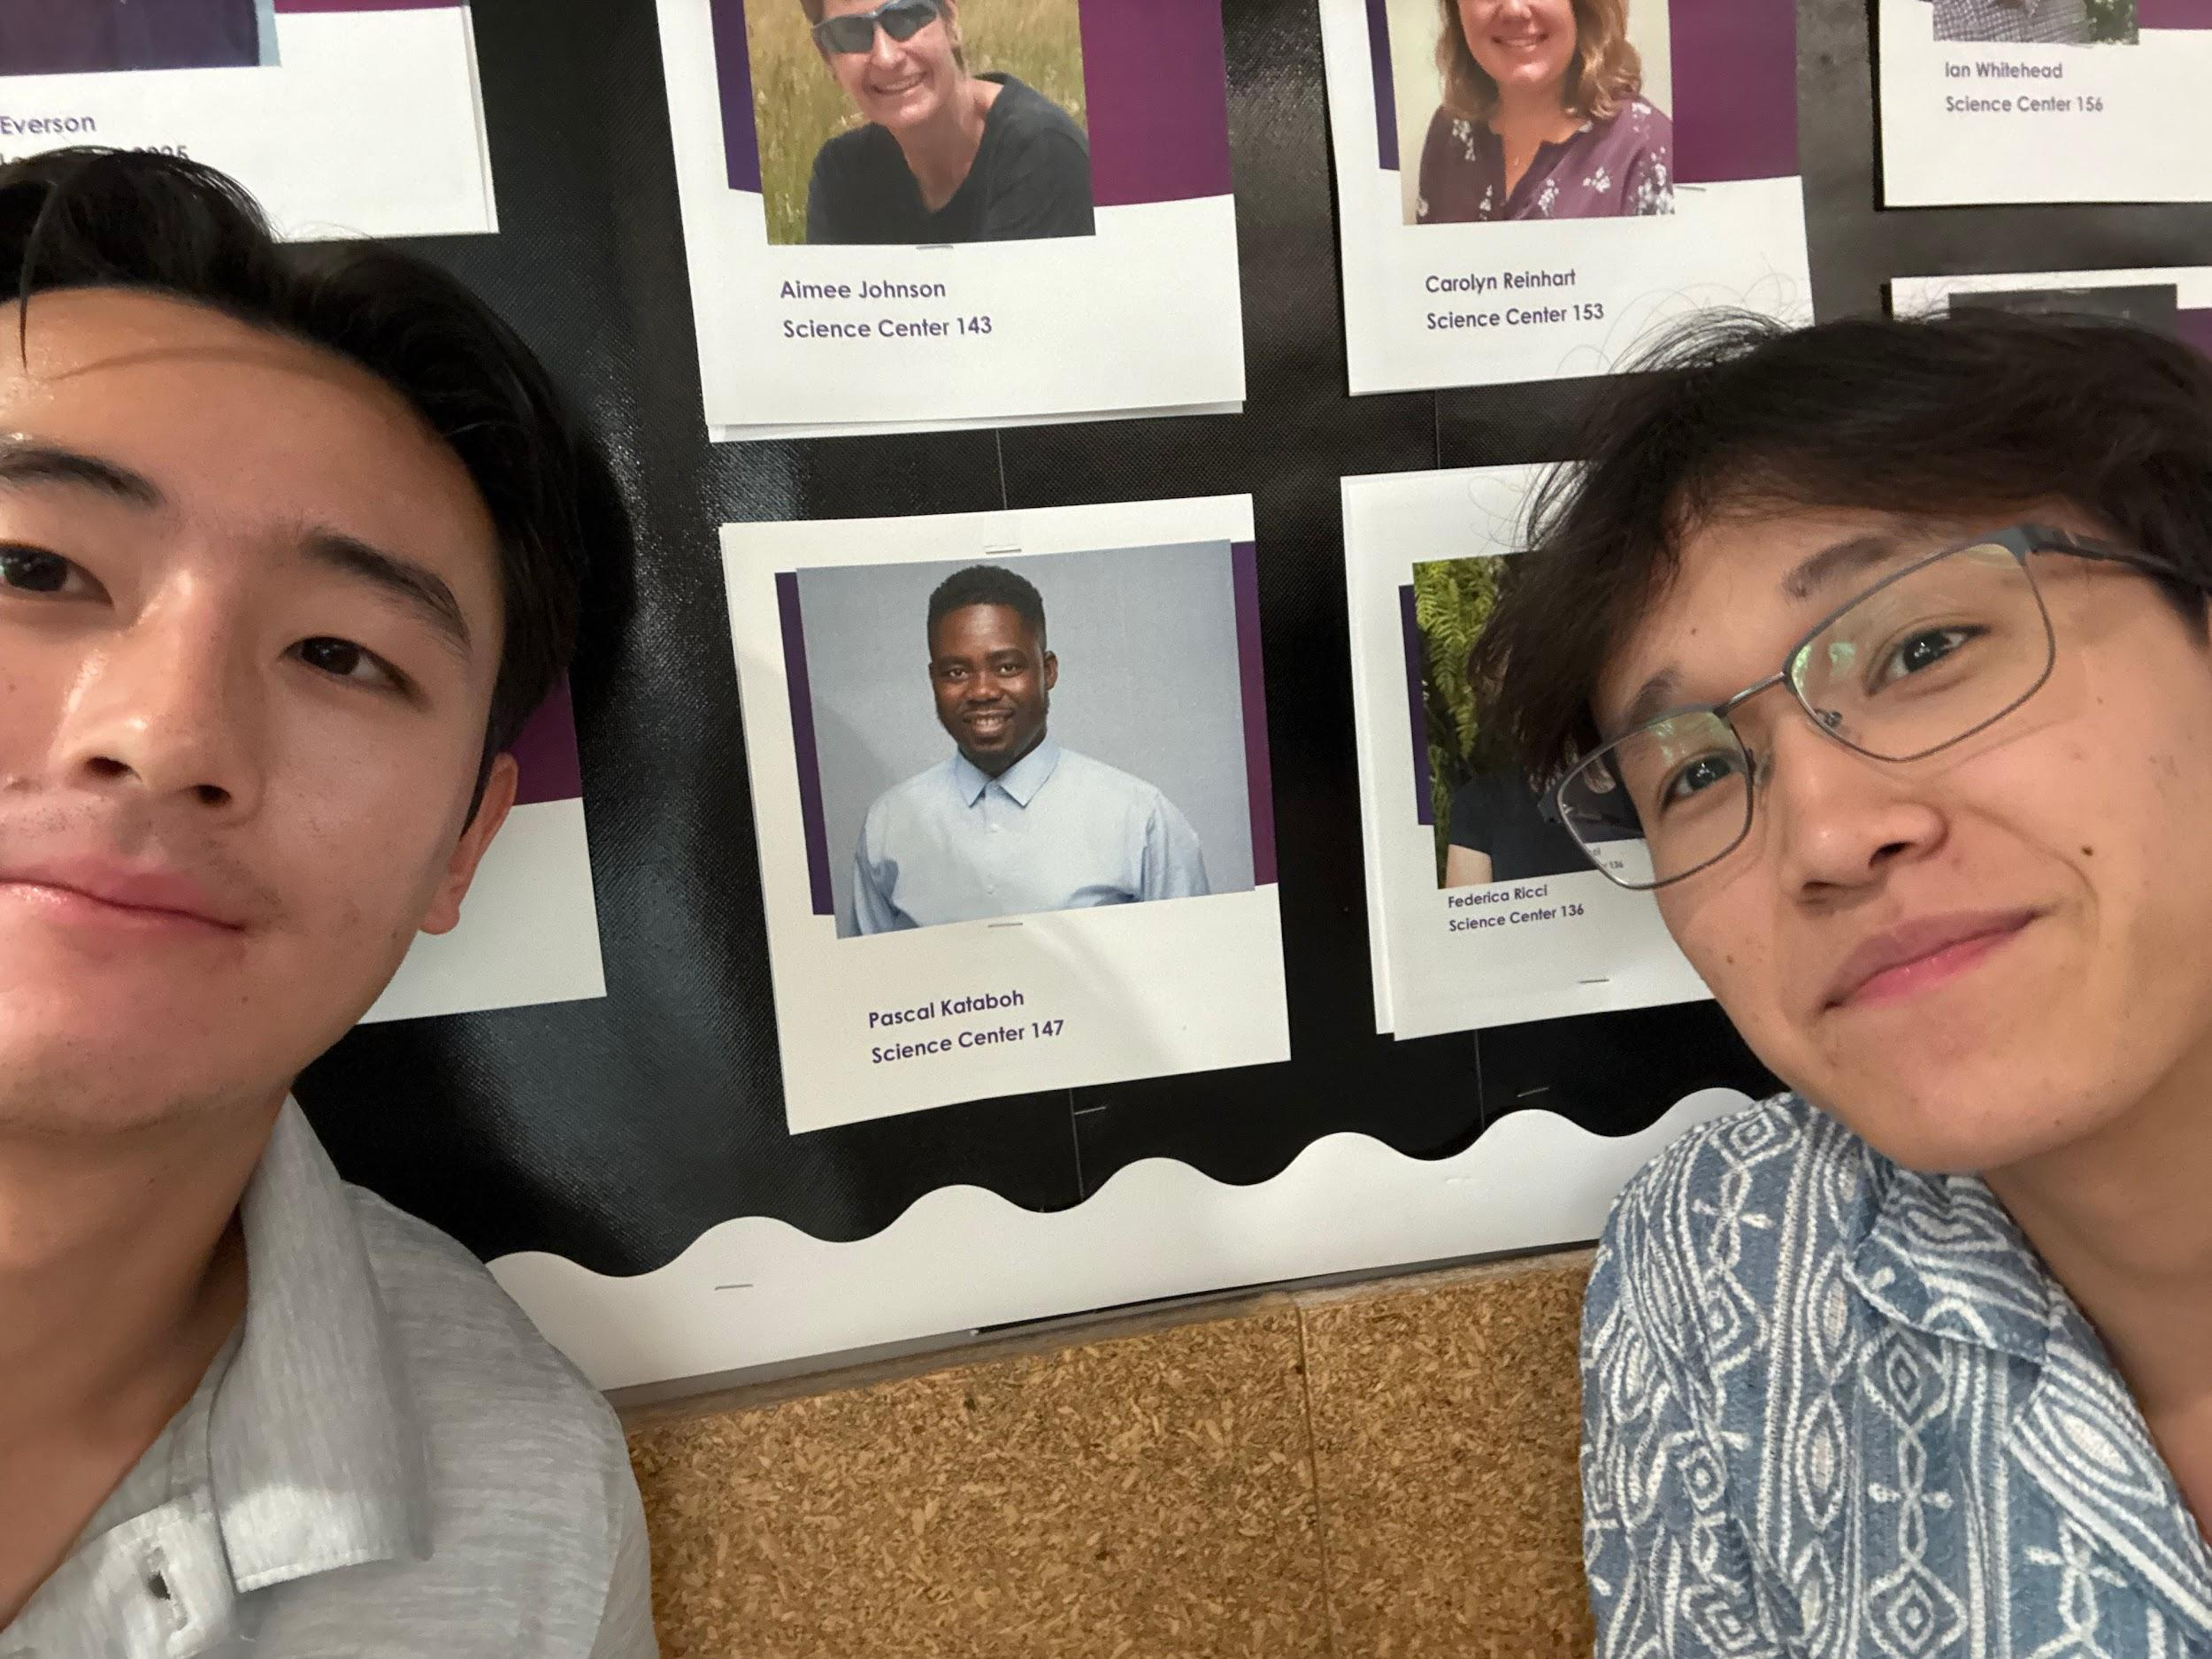
\includegraphics[width=0.92\linewidth]{assets/source_selfie.jpg}\par
      \vspace{0.12cm}
      {\scriptsize Thank you very much to the \textbf{Provost's Office} for funding our summer research project!}
    \end{column}
  \end{columns}
\end{frame}

\end{document}
